\section{Diffractive scattering}%
\label{sec:diffraction}

\subsection{Moment decomposition}%
\label{sec:diffraction:moment}

One of the simplest reactions to study excited mesons is the
production of a system of two distinguishable spinless particles in
the strong interaction of a highly energetic beam meson (usually
pion or kaon) with a stationary nucleon or nuclear target.  We are
interested in the short-lived intermediate mesonic states~$X$
(resonances) that are produced in these reactions and that decay into
the observed two-(pseudo)scalar system.  A typical example for such a
process is the reaction
\begin{equation}
  \pi^-\, p \to X^-\, p \to \etaOrPrPim\, p,
\end{equation}
which is shown in \cref{fig:diffraction_etaprimepi}.  How to analyze
these reactions was studied in detail by S.U.~Chung in
\refCite{Chung:1997qd}.  We will follow this reference here and will
derive some equations.

\begin{figure}[bp]
  \centering%
  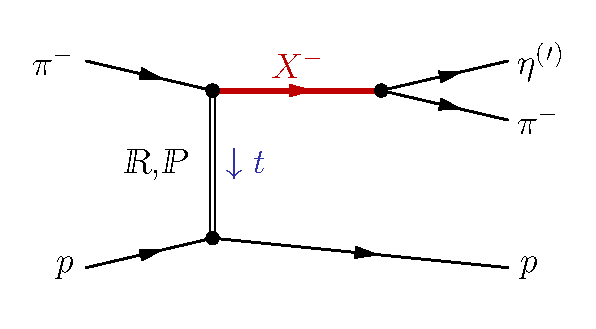
\includegraphics[width=0.5\textwidth]{diffractive_dissociation_x_etaprimepi_charged_p}%
  \caption{Diffractive scattering of a beam pion off a target proton
  mediated by Reggeon exchange.  In this scattering process, an
  intermediate state~$X^-$ with well-defined quantum numbers is
  produced, which in the example given here decays into the
  \etaOrPrPim channel.}%
  \label{fig:diffraction_etaprimepi}%
\end{figure}

The analysis is based on the intensity distribution, \ie the number
density distribution of events produced in the studied inelastic
scattering reaction, which we decompose into partial-wave
amplitudes:\footnote{This is the simplest possible formula, were we
assume that the effect of the target spin is negligible and that all
partial wave amplitudes are fully coherent.}
\begin{equation}
  \label{eq:diffraction_intensity}
  \intensity(\Omega; w, t)
  = \frac{\dif{N}}{\dif{w}\, \dif{t}\, \dif{\Omega}}
  = \Abs[3]{\sum_{\ell m}^\infty \prodAmp_{\ell\, m}(w, t)\, Y_\ell^m(\Omega)}^2
  = \sum_{\substack{\ell m \\ \ell' m'}}^\infty Y_\ell^m(\Omega)\, \varrho^{\ell\, \ell'}_{m\, m'}(w, t)\, Y_{\ell'}^{m' *}(\Omega).
\end{equation}
Here, $N$~is the number of produced events,\footnote{In an analysis of
measured data, this would correspond to the acceptance-corrected
number of measured events.} $w$~is the invariant mass of the
two-(pseudo)scalar system, $t$~is the squared four-momentum
transferred from the beam to the target particle, and $\Omega =
(\theta, \phi)$ is the direction of one of the two (pseudo)scalar
mesons the~$X$ decays into, measured in the Gottfried-Jackson rest
frame of~$X$.  The $\prodAmp_{\ell\, m}(w, t)$ are the partial-wave
amplitudes that correspond to an intermediate state with a spin given
by the relative orbital angular momentum~$\ell$ between the
two-(pseudo)scalar mesons and a spin projection~$m$ \wrt the beam
axis.  The partial-wave amplitudes form the spin-density matrix
of~$X$:
\begin{equation}
  \label{eq:diffraction_spin_dens_def}
  \varrho^{\ell\, \ell'}_{m\, m'}(w, t)
  = \prodAmp_{\ell\, m}(w, t)\, \prodAmp_{\ell'\, m'}^*(w, t),
\end{equation}
which by definition is Hermitian.  The angular distribution of the
$X$~decay products is given by the spherical harmonics
$Y_\ell^m(\Omega)$~\cite{wikipedia:sphericalHarm}, which are defined
by\footnote{See Eq.~(1) in Sec.~5.2 of
\refCite{Varshalovich:1988krb}.}
\begin{equation}
  \label{eq:spherical_harm_def}
  Y_\ell^m(\Omega)
  = \dUnderbrace{\sqrt{\frac{(2 \ell + 1)}{4 \pi}\, \frac{(\ell -m)!}{(\ell + m)!}}\, P_\ell^m(\cos\theta)}{= Y_\ell^m(\theta, 0)}\, e^{\imag\, m\, \phi},
\end{equation}
For convenience, we introduce the real-valued functions
\begin{equation}
  \label{eq:small_y_def}
  y_\ell^m(\theta)
  \equiv Y_\ell^m(\theta, 0)
  \quad\text{so that}\quad
  Y_\ell^m(\theta, \phi)
  = y_\ell^m(\theta)\, e^{\imag\, m\, \phi}.
\end{equation}
The spherical harmonics are special cases of the
$D$-functions~\cite{wikipedia:wignerD}, \ie\footnote{See Eq.~(37) in
Sec.~5.2.7 of \refCite{Varshalovich:1988krb}.}
\begin{equation}
  \label{eq:spherical_harm_wigner_d}
  Y_\ell^m(\Omega)
  = \sqrt{\frac{2 \ell + 1}{4 \pi}}\, D^{\ell *}_{m 0}(\phi, \theta, 0)
  \quad\text{and in particular}\quad
  y_\ell^m(\theta)
  = \sqrt{\frac{2 \ell + 1}{4 \pi}}\, d^\ell_{m 0}(\theta).
\end{equation}
They obey the integral relation (see Eq.~(1) in Sec.~5.9 of
\refCite{Varshalovich:1988krb})
\begin{equation}
  \label{eq:spherical_harmonics_integral}
  \int_{4 \pi}\!\!\!\! \dif{\Omega}\, Y_\ell^m(\Omega)
  = \sqrt{4 \pi}\, \delta_{\ell 0}\, \delta_{m 0}.
\end{equation}

In a partial-wave analysis, the partial-wave amplitudes
$\prodAmp_{\ell\, m}$, which contain the information about the
produced resonances~$X$, are determined by fitting the intensity model
in \cref{eq:diffraction_intensity} to the measured
$\Omega$~distribution in narrow $(w, t)$ cells taking into account the
experimental acceptance.  Within each kinematic cell,
$\prodAmp_{\ell\, m}$ is treated as constant.  To simplify notation,
we hence will omit the~$w$ and $t$~dependencies in all formulas below.

In addition to the partial-wave analysis, which decomposes the
\emph{amplitudes} into spherical harmonics, we can exploit the fact
that the $Y_\ell^m(\Omega)$ constitute a complete orthonormal set of
base functions on the surface of a unit sphere, \ie they fullfil the
completeness relation\footnote{See Eq.~(1) in Sec.~5.6.1 of
\refCite{Varshalovich:1988krb}.}
\begin{equation}
  \label{eq:spherical_harm_complete}
  \sum_{\ell m}^\infty Y_\ell^m(\Omega)\, Y_\ell^{m *}(\Omega')
  = \delta(\phi' - \phi)\, \delta(\theta' - \theta)
\end{equation}
and the orthonormality relation\footnote{%
Throughout the text, we use
\begin{equation}
  \int_{-1}^{+1}\!\!\! \dif{\cos\theta} \int_{-\pi}^{+\pi}\!\!\! \dif{\phi}
  = \int_{4 \pi}\!\!\!\! \dif{\Omega}.
\end{equation}
}\footnote{See Eq.~(2) in Sec.~5.6.1 of
\refCite{Varshalovich:1988krb}.}
\begin{equation}
  \label{eq:spherical_harm_orthonorm}
  \int_{4 \pi}\!\!\!\! \dif{\Omega}\, Y_\ell^m(\Omega)\, Y_{\ell'}^{m' *}(\Omega)
  = \delta_{\ell \ell'}\, \delta_{m m'},
\end{equation}
and instead decompose the \emph{intensity} into spherical harmonics.

Using \cref{eq:gen_fourier_series,eq:expansion_coefficient} we
obtain:\footnote{The expansion into a series of spherical harmonics is
also referred to as Laplace series~\cite{MathWorld:LaplaceSeries}.}
\begin{equation}
  \label{eq:diffraction_intensity_moments}
  \intensity(\Omega)
  = \sum_{L M}^\infty H(L, M)\, Y_L^M(\Omega),
\end{equation}
with the moments\footnote{Note that in
\cref{sec:diffraction:moments_norm}, we will introduce a different
normalization for $H(L, M)$ (see \cref{eq:diffraction_moments_norm}).}
\begin{equation}
  \label{eq:diffraction_moments}
  H(L, M)
  = \int_{4 \pi}\!\!\!\! \dif{\Omega}\, \intensity(\Omega)\, Y_L^{M *}(\Omega).
\end{equation}
It is important to note that although
\cref{eq:diffraction_intensity_moments} and
\cref{eq:diffraction_intensity} use the same basis functions, the two
represent different decompositions.  In
\cref{eq:diffraction_intensity} the amplitudes are decomposed into
spherical harmonics, \ie partial-wave amplitudes, whereas in
\cref{eq:diffraction_intensity_moments} the intensity is decomposed.
Whereas the former decomposition is based on a physics model of the
reaction, the moment decomposition is purely mathematical.  An
advantage of the moment decomposition is that it is unique, whereas
the partial-wave decomposition may have mathematical as well as
statistical ambiguities (see \eg\ \refCite{Chung:1997qd}).  Another
advantage of the moment decomposition is that the moments can be
rather easily calculated from the data, which will be discussed in
\cref{sec:diffraction:moments_data}.  The downside of this approach is
that the physics interpretation of the moments is difficult because
they are only indirectly related to the partial-wave amplitudes.  This
will be discussed in more detail in \cref{sec:diffraction:moments_pw}.


\subsection{Relation between moments and partial-wave amplitudes}%
\label{sec:diffraction:moments_pw}

In order to relate the partial-wave amplitudes~$\prodAmp_{\ell\,
m}$ and the moments~$H(L, M)$ we express the moments in terms of
spin-density elements using the relation\footnote{See Eq.~(A.15) in
\refCite{Chung:1971ri}.}
\begin{equation}
  \label{eq:spherical_harm_prod}
  Y_{\ell'}^{m' *}(\Omega)\, Y_{\ell}^m(\Omega)
  = \sum_{L M}^\infty \sqrt{\frac{2 L + 1}{4 \pi}}\, \sqrt{\frac{2 \ell' + 1}{2 \ell + 1}}\, \clebsch{\ell'}{0}{L}{0}{\ell}{0}\, \clebsch{\ell'}{m'}{L}{M}{\ell}{m}\, Y_L^M(\Omega).
\end{equation}
Here, \clebsch{j_1}{m_1}{j_2}{m_2}{J}{M} are the Clebsch-Gordan
coefficients for the coupling of the spin states $\ket{j_1\; m_1}$
and~$\ket{j_2\; m_2}$ to $\ket{J\; M}$.  Note that the Clebsch-Gordan
coefficient \clebsch{\ell'}{0}{L}{0}{\ell}{0} requires
that\footnote{See Eq.~(32) in Sec.~8.5.2 of
\refCite{Varshalovich:1988krb}.}
\begin{equation}
  \label{eq:ang_mom_sum}
  \ell' + L + \ell
  = \text{even}.
\end{equation}
Inserting \cref{eq:spherical_harm_prod} into
\cref{eq:diffraction_intensity}, yields
\begin{equation}
  \intensity(\Omega)
  = \sum_{L M}^\infty \sqrt{\frac{2 L + 1}{4 \pi}} \sum_{\substack{\ell m \\ \ell' m'}}^\infty
  \sqrt{\frac{2 \ell' + 1}{2 \ell + 1}}\, \clebsch{\ell'}{0}{L}{0}{\ell}{0}\, \clebsch{\ell'}{m'}{L}{M}{\ell}{m}\,
  \varrho^{\ell\, \ell'}_{m\, m'}\, Y_L^M(\Omega).
\end{equation}
Comparing with \cref{eq:diffraction_intensity_moments}, we see
that\footnote{Note that in \cref{sec:diffraction:moments_norm}, we
will introduce a different normalization for $H(L, M)$ (see
\cref{eq:diffraction_moments_pw_norm}).}
\begin{equation}
  \label{eq:diffraction_moments_pw}
  H(L, M)
  = \sqrt{\frac{2 L + 1}{4 \pi}} \sum_{\substack{\ell m \\ \ell' m'}}^\infty
  \sqrt{\frac{2 \ell' + 1}{2 \ell + 1}}\,
  \clebsch{\ell'}{0}{L}{0}{\ell}{0}\, \clebsch{\ell'}{m'}{L}{M}{\ell}{m}\,
  \varrho^{\ell\, \ell'}_{m\, m'}.
\end{equation}

It is important to note that we can always calculate all moments from
a given set of partial-wave amplitudes using
\cref{eq:diffraction_moments_pw}.  However, in general the converse is
not true because there are unphysical sets of moments that do not
correspond to a partial-wave decomposition and even for a physical set
of moments we need to solve a system of quadratic equations in the
partial-wave amplitudes given by
\cref{eq:diffraction_moments_pw,eq:diffraction_spin_dens_def}, which
may contain ambiguities.

From \cref{eq:diffraction_moments_pw} it is clear that the moments are
linear combinations of spin-density matrix elements, \ie of
intensities and interference terms of the partial-wave amplitudes
$\prodAmp_{\ell\, m}$.  The equation also shows that~$L$ and~$M$
are only indirectly linked to the physical angular momentum quantum
numbers of the two-body system.  For given~$L$, the Clebsch-Gordan
coefficients limit the sum to those partial waves, for which $\ell' +
L + \ell = \text{even}$ (see \cref{eq:ang_mom_sum}), $\abs{\ell' - L}
\leq \ell \leq \ell' + L$, and $m = m' + M$.  This means that if the
partial-wave amplitudes vanish for $\ell, \ell' > \ell_\text{max}$ the
moments~$H(L, M)$ will vanish $L > 2 \ell_\text{max}$.

Alternatively, we can derive \cref{eq:diffraction_moments_pw} by
inserting \cref{eq:diffraction_intensity} into
\cref{eq:diffraction_moments}.  Doing so, we obtain
\begin{equation}
  H(L, M)
  = \sum_{\substack{\ell m \\ \ell' m'}}^\infty
  \varrho^{\ell\, \ell'}_{m\, m'}\,
  \int_{4 \pi}\!\!\!\! \dif{\Omega}\,
  Y_\ell^m(\Omega)\,
  Y_{\ell'}^{m' *}(\Omega)\,
  Y_L^{M *}(\Omega).
\end{equation}
Using\footnote{This is the complex conjugate of Eq.~(4) in Sec.~5.9.1
of \refCite{Varshalovich:1988krb}.}
\begin{equation}
  \label{eq:spherical_harm_clebsch}
  \int_{4 \pi}\!\!\!\! \dif{\Omega}\,
  Y_{\ell'}^{m' *}(\Omega)\, Y_L^{M *}(\Omega)\, Y_{\ell}^m(\Omega)
  = \sqrt{\frac{2 \ell' + 1}{4 \pi}}\, \sqrt{\frac{2 L + 1}{2 \ell + 1}}\, \clebsch{\ell'}{0}{L}{0}{\ell}{0}\, \clebsch{\ell'}{m'}{L}{M}{\ell}{m},
\end{equation}
this is equivalent to \cref{eq:diffraction_moments_pw}.


\subsection{Normalization of moments}%
\label{sec:diffraction:moments_norm}

A more practical normalization of the moments is obtained by the
redefinition
\begin{equation}
  H(L, M)
  \to \sqrt{\frac{2 L + 1}{4 \pi}}\, H(L, M).
\end{equation}
Applying the above,
\cref{eq:diffraction_intensity_moments,eq:diffraction_moments} become
\begin{equation}
  \label{eq:diffraction_intensity_moments_norm}
  \intensity(\Omega)
  = \sum_{L M}^\infty \sqrt{\frac{2 L + 1}{4 \pi}}\, H(L, M)\, Y_L^M(\Omega),
\end{equation}
and
\begin{equation}
  \label{eq:diffraction_moments_norm}
  H(L, M)
  = \sqrt{\frac{4 \pi}{2 L + 1}}\, \int_{4 \pi}\!\!\!\! \dif{\Omega}\, \intensity(\Omega)\, Y_L^{M *}(\Omega).
\end{equation}
Using the relation between the spherical harmonics and the Wigner
$D$-functions in \cref{eq:spherical_harm_wigner_d},
\cref{eq:diffraction_intensity_moments_norm,eq:diffraction_moments_norm}
become identical to Eqs.~(6) and~(9) in \refCite{Chung:1997qd}.

This normalization gives a direct interpretation to the lowest moment
$H(0, 0)$.  According to \cref{eq:diffraction_intensity},
$\intensity(\Omega)$ is the number density distribution of produced
events.  Consequently, integrating $\intensity(\Omega)$ over the full
solid angle $4 \pi$ gives the total number~$N$ of events produced in
the considered $\omega$~and $t$~ranges:
\begin{align}
  \label{eq:diffraction_intensity_norm}
  N
  ={}& \int_{4 \pi}\!\!\!\! \dif{\Omega}\, \intensity(\Omega)
  \\
  ={}& \int_{4 \pi}\!\!\!\! \dif{\Omega}\, \sum_{L M}^\infty \sqrt{\frac{2 L + 1}{4 \pi}}\, H(L, M)\, Y_L^M(\Omega)
  \\
  ={}& \sum_{L M}^\infty \sqrt{\frac{2 L + 1}{4 \pi}}\, H(L, M)\,
  \rdUnderbrace{\int_{4 \pi}\!\!\!\! \dif{\Omega}\, Y_L^M(\Omega)}%
  {\equalUsing{\cref{eq:spherical_harmonics_integral}} \sqrt{4 \pi}\, \delta_{L 0}\, \delta_{M 0}}
  \\
  \label{eq:diffraction_H00_norm}
  ={}& H(0, 0) \in \mathbb{R}.
\end{align}
Here, we have inserted \cref{eq:diffraction_intensity_moments_norm} in
the first step.  This is consistent with the definition of $H(0, 0)$
in \cref{eq:diffraction_moments_norm}:
\begin{equation}
  H(0, 0)
  = \sqrt{4 \pi}\, \int_{4 \pi}\!\!\!\! \dif{\Omega}\, \intensity(\Omega)\, \cdUnderbrace{Y_0^{0 *}(\Omega)}{= 1 / \sqrt{4 \pi}}
  = \int_{4 \pi}\!\!\!\! \dif{\Omega}\, \intensity(\Omega)
  = N.
\end{equation}

The normalization in \cref{eq:diffraction_moments_norm} also
simplifies \cref{eq:diffraction_moments_pw}, which becomes
\begin{equation}
  \label{eq:diffraction_moments_pw_norm}
  H(L, M)
  = \sum_{\substack{\ell m \\ \ell' m'}}^\infty
  \sqrt{\frac{2 \ell' + 1}{2 \ell + 1}}\,
  \clebsch{\ell'}{0}{L}{0}{\ell}{0}\, \clebsch{\ell'}{m'}{L}{M}{\ell}{m}\,
  \varrho^{\ell\, \ell'}_{m\, m'}.
\end{equation}
Using
\begin{equation}
  \clebsch{\ell'}{m'}{0}{0}{\ell}{m}
  = \delta_{\ell \ell'}\, \delta_{m m'},
\end{equation}
we see in particular that $H(0, 0)$ is identical to the sum of all
partial-wave intensities, which are given by the diagonal elements of
the spin-density matrix:
\begin{equation}
  \label{eq:diffraction_moment_00_pw}
  H(0, 0)
  = \sum_{\substack{\ell m \\ \ell' m'}}^\infty
  \sqrt{\frac{2 \ell' + 1}{2 \ell + 1}}\, \delta_{\ell \ell'}\, \delta_{m m'}\, \varrho^{\ell\, \ell'}_{m\, m'}
  = \sum_{\ell m}^\infty \varrho^{\ell\, \ell}_{m\, m}.
\end{equation}

For the remainder of this section we will use the moments defined in
\cref{eq:diffraction_intensity_moments_norm,eq:diffraction_moments_norm,eq:diffraction_moments_pw_norm}.


\subsection{Symmetry properties of moments}%
\label{sec:diffraction:moments_sym}

Since the moments are defined by the spherical harmonics (see
\cref{eq:diffraction_moments_norm}), they inherit the symmetry properties
of the spherical harmonics.  From\footnote{See Eq.~(1) in Sec.~5.4 of
\refCite{Varshalovich:1988krb}.}
\begin{equation}
  \label{eq:spherical_harm_sym}
  Y_L^{M *}(\Omega)
  = (-1)^M\, Y_L^{(-M)}(\Omega)
\end{equation}
it follows that
\begin{equation}
  \label{eq:diffraction_moment_sym_1}
  H^*(L, M)
  = \sqrt{\frac{4 \pi}{2 L + 1}}\, \int_{4 \pi}\!\!\!\! \dif{\Omega}\, \intensity(\Omega)\, Y_L^M(\Omega)
  = (-1)^M \sqrt{\frac{4 \pi}{2 L + 1}}\, \int_{4 \pi}\!\!\!\! \dif{\Omega}\, \intensity(\Omega)\, Y_L^{(-M) *}(\Omega)
  = (-1)^M\, H(L, -M).
\end{equation}

Alternatively, we can derive \cref{eq:diffraction_moment_sym_1} by
using \cref{eq:diffraction_moments_pw_norm} plus the fact that the
spin-density matrix is Hermitian,
\ie
\begin{equation}
  \rBrk[1]{\varrho^{\ell\, \ell'}_{m\, m'}}^*
  = \varrho^{\ell'\, \ell}_{m'\, m},
\end{equation}
and that the Clebsch-Gordan coefficients have the symmetry
property\footnote{See Eq.~(10) in Sec.~8.4.3 of
\refCite{Varshalovich:1988krb}.}
\begin{equation}
  \label{eq:clebsch_sym}
  \clebsch{\ell'}{m'}{L}{M}{\ell}{m}
  = \rdUnderbrace{(-1)^{\ell' + L - \ell}}{\equalUsing{$\mathclap{\text{\cref{eq:ang_mom_sum}}}$}\quad 1}\,
  \clebsch{L}{M}{\ell'}{m'}{\ell}{m}
  = (-1)^{L - M}\, \sqrt{\frac{2 \ell + 1}{2 \ell' + 1}}\, \clebsch{\ell}{m}{L}{-M}{\ell'}{m'}.
\end{equation}
Doing so, we get
\begin{align}
  H^*(L, M)
  ={}& \sum_{\substack{\ell m \\ \ell' m'}}^\infty
    \sqrt{\frac{2 \ell' + 1}{2 \ell + 1}}\,
    (-1)^{L - 0}\, \sqrt{\frac{2 \ell + 1}{2 \ell' + 1}}\, \clebsch{\ell}{0}{L}{0}{\ell'}{0}\,
    (-1)^{L - M}\, \sqrt{\frac{2 \ell + 1}{2 \ell' + 1}}\, \clebsch{\ell}{m}{L}{-M}{\ell'}{m'}\,
    \varrho^{\ell'\, \ell}_{m'\, m} \nonumber
  \\
  ={}& \dUnderbrace{(-1)^{2 L - M}}{= (-1)^M}
  \sum_{\substack{\ell m \\ \ell' m'}}^\infty
  \sqrt{\frac{2 \ell + 1}{2 \ell' + 1}}\,
  \clebsch{\ell}{0}{L}{0}{\ell'}{0}\, \clebsch{\ell}{m}{L}{-M}{\ell'}{m'}\,
  \varrho^{\ell'\, \ell}_{m'\, m}
  \\
  \equalUsing{$\mathclap{\substack{\displaystyle{\ell \leftrightarrow \ell'} \\ \displaystyle{m \leftrightarrow m'}}}$}{}& \quad
  (-1)^M\, H(L, -M),
\end{align}
where in the last step we rearranged the terms in the sum and compared
to \cref{eq:diffraction_moments_pw_norm}.

The symmetry relation in \cref{eq:diffraction_moment_sym_1} ensures
that the intensity function in
\cref{eq:diffraction_intensity_moments_norm} is real-valued:
\begin{flalign}
  \intensity(\Omega)
  ={}& \sum_{L = 0}^\infty \sum_{M = -L}^{+L} \sqrt{\frac{2 L + 1}{4 \pi}}\, H(L, M)\, Y_L^M(\Omega) && \nonumber
  \\
  ={}& \sum_{L = 0}^\infty \sqrt{\frac{2 L + 1}{4 \pi}} \sBrk[4]{\rdUnderbrace{\sum_{M = -L}^{-1} H(L, M)\, Y_L^M(\Omega)}%
    {= \sum_{M = +1}^{+L} H(L, -M)\, Y_L^{(-M)}(\Omega)
    \equalUsingTwo{\cref{eq:spherical_harm_sym}}{\cref{eq:diffraction_moment_sym_1}} (-1)^M\, H^*(L, M)\, (-1)^M\, Y_L^{M *}(\Omega)}
    + H(L, 0)\, Y_L^0(\Omega) + \sum_{M = +1}^{+L} H(L, M)\, Y_L^M(\Omega)} && \nonumber
  \\
  ={}& \sum_{L = 0}^\infty \sqrt{\frac{2 L + 1}{4 \pi}} \sBrk[4]{H(L, 0)\, Y_L^0(\Omega) + \sum_{M = +1}^{+L}
  \rdUnderbrace{\cBrk{H(L, M)\,Y_L^M(\Omega) + H^*(L, M)\,Y_L^{M *}(\Omega)}}{= 2 \Re{H(L, M)\, Y_L^M(\Omega)}}} && \nonumber
  \\
  \label{eq:diffraction_intensity_moments_general}
  ={}& \sum_{L = 0}^\infty \sqrt{\frac{2 L + 1}{4 \pi}} \sum_{M = 0}^{L} (2 - \delta_{M 0})\, \Re{H(L, M)\, Y_L^M(\Omega)}. &&
\end{flalign}
For the last step, we have used that $Y_L^0(\Omega)$ and hence also
$H(L, 0)$ are real-valued by construction.  Due to the above, we only
have to calculate the moments with $M \geq 0$.

In addition to the symmetry properties of the spherical harmonics, we
can also exploit the symmetry properties of the $X$~spin-density
matrix.  Since the scattering process is invariant under parity, we
have\footnote{See Eq.~2.7 in \refCite{Chung:1974fq}.}
\begin{equation}
  \label{eq:diffraction_spin_dens_parity_general}
  \varrho^{\ell\, \ell'}_{m\, m'}
  = P\, P'\, (-1)^{\ell - \ell'}\, (-1)^{m - m'}\, \varrho^{\ell'\, \ell}_{{-m}\, {-m'}}.
\end{equation}
Here $\ell^P$ and $(\ell')^{P'}$ are two spin-parity states of~$X$.
For the two-body decay $X \to 1 + 2$, the intrinsic parity of~$X$ is
given by
\begin{equation}
  P
  = P_1\, P_2\, (-1)^\ell.
\end{equation}
Assuming that $X$~decays into two daughter particles with identical
parity, \eg two pseudoscalars such as $\etaOrPr \pi$,
\cref{eq:diffraction_spin_dens_parity_general} simplifies to
\begin{equation}
  \label{eq:diffraction_spin_dens_parity}
  \varrho^{\ell\, \ell'}_{m\, m'}
  = (-1)^{m - m'}\, \varrho^{\ell'\, \ell}_{{-m}\, {-m'}}.
\end{equation}

Using this together with
\cref{eq:diffraction_moments_pw_norm} and the symmetry
property\footnote{See Eq.~(11) in Sec.~8.4.3 of
\refCite{Varshalovich:1988krb}.}
\begin{equation}
  \label{eq:clebsch_sym2}
  \clebsch{\ell'}{m'}{L}{M}{\ell}{m}
  = \rdUnderbrace{(-1)^{\ell' + L - \ell}}{\equalUsing{$\mathclap{\text{\cref{eq:ang_mom_sum}}}$}\quad 1}\,
  \clebsch{\ell'}{-m'}{L}{-M}{\ell}{-m}
\end{equation}
of the Clebsch-Gordan coefficients, we get
\begin{align}
  H(L, -M)
  ={}& \sum_{\substack{\ell m \\ \ell' m'}}^\infty
  \sqrt{\frac{2 \ell' + 1}{2 \ell + 1}}\,
  \clebsch{\ell'}{0}{L}{0}{\ell}{0}\, \clebsch{\ell'}{-m'}{L}{M}{\ell}{-m}\,
  (-1)^{m - m'}\, \varrho^{\ell\, \ell'}_{{-m}\, {-m}'} \nonumber
  \\
  \label{eq:diffraction_moment_sym_2}
  \equalUsing{$\mathclap{\substack{\displaystyle{m \to -m} \\ \displaystyle{m' \to -m'}}}$}{}& \quad
  (-1)^M\, H(L, M),
\end{align}
where in the last step, we used that the second Clebsch-Gordan
coefficient enforces $m' - M = m$,\footnote{Therefore, $(-1)^{m - m'}
= (-1)^{m' - m} = (-1)^M$.} rearranged the terms in the sum, and
compared to \cref{eq:diffraction_moments_pw_norm}.

From \cref{eq:diffraction_moment_sym_1,eq:diffraction_moment_sym_2} follows that
\begin{equation}
  \label{eq:diffraction_moment_real}
  H(L, M)
  = H^*(L, M),
\end{equation}
\ie all moments must be real-valued.  Inserting
\cref{eq:small_y_def,eq:diffraction_moments_norm} on both sides, we
obtain
\begin{align}
  \sqrt{\frac{4 \pi}{2 L + 1}}\, \int_{4 \pi}\!\!\!\! \dif{\Omega}\, \intensity(\Omega)\, Y_L^{M *}(\Omega)
  \mustBeEq{}&
  \sqrt{\frac{4 \pi}{2 L + 1}}\, \int_{4 \pi}\!\!\!\! \dif{\Omega}\, \intensity(\Omega)\, Y_L^M(\Omega) \\
  \sqrt{\frac{4 \pi}{2 L + 1}}\, \int_{4 \pi}\!\!\!\! \dif{\Omega}\, \intensity(\Omega)\, y_L^M(\theta) \sBrk[2]{\cos(M \phi) - \imag \sin(M \phi)}
  \mustBeEq{}&
  \sqrt{\frac{4 \pi}{2 L + 1}}\, \int_{4 \pi}\!\!\!\! \dif{\Omega}\, \intensity(\Omega)\, y_L^M(\theta) \sBrk[2]{\cos(M \phi) + \imag \sin(M \phi)},
\end{align}
wich must hold for all $\Omega = (\theta, \phi)$.  Consequently,
\begin{align}
  \label{eq:diffraction_moments_imag}
  0
  \mustBeEq{}& \sqrt{\frac{4 \pi}{2 L + 1}}\, \int_{4 \pi}\!\!\!\! \dif{\Omega}\, \intensity(\Omega)\, y_L^M(\theta)\, \sin(M\, \phi)
  \intertext{and hence}
  \label{eq:diffraction_moments_real}
  H(L, M)
  \mustBeEq{}& \sqrt{\frac{4 \pi}{2 L + 1}}\, \int_{4 \pi}\!\!\!\! \dif{\Omega}\, \intensity(\Omega)\, y_L^M(\theta)\, \cos(M\, \phi) \quad \in \mathbb{R}.
\end{align}

Using the above, we can rewrite \cref{eq:diffraction_intensity_moments_general}:
\begin{align}
  \intensity(\Omega)
  ={}& \sum_{L = 0}^\infty \sqrt{\frac{2 L + 1}{4 \pi}} \sum_{M = 0}^{L} (2 - \delta_{M 0})\, \Re[2]{H(L, M)}\, \Re[2]{Y_L^M(\Omega)} \nonumber
  \\
  \label{eq:diffraction_intensity_moments_real}
  ={}& \sum_{L = 0}^\infty \sqrt{\frac{2 L + 1}{4 \pi}} \sum_{M = 0}^{L} (2 - \delta_{M 0})\, H(L, M)\, y_L^M(\theta)\, \cos(M\, \phi).
\end{align}
This is identical to Eq.~(13) in \refCite{Chung:1997qd} and means that
parity requires the intensity to be an even function in~$\phi$.


\subsection{Reflectivity basis}%
\label{sec:diffraction:reflectivity}

It is often advantageous to express the intensity distribution in
\cref{eq:diffraction_intensity} in the reflectivity basis, \ie using
the reflectivity states of~$X$
\begin{equation}
  \label{eq:diffraction_refl_def}
  \ket{\refl, \ell, m}
  \equiv \mathcal{N}_m \sBrk[2]{\ket{\ell, m} - \refl\, (-1)^m\, \ket{\ell, {-m}}},
\end{equation}
which are eigenstates of the reflection operator~$\Pi_y$ through the
production plane that is spanned by the momenta of the beam particle
and~$X$.  The relative sign of the terms in
\cref{eq:diffraction_refl_def} has been chosen such that for a
pseudoscalar beam particle the eigenvalues~$\refl = \pm$ of~$\Pi_y$,
\ie the \emph{reflectivities}, correspond to the \emph{naturality} of
the exchange particle in the scattering process.  The normalization
factor
\begin{equation}
  \label{eq:refl_norm}
  \mathcal{N}_m
  = \begin{cases*}
      1 / \sqrt{2} & for $m > 0$, \\
      1 / 2        & for $m = 0$, \\
      0            & for $m < 0$
    \end{cases*}
\end{equation}
ensures that the multiplicity of $2 \ell + 1$ of the spin states is
conserved by constraining~$m$ to be non-negative.  It is important to
note that the definition in \cref{eq:diffraction_refl_def} forbids
positive-reflectivity states with $m = 0$.

The reflectivity basis is implemented by introducing the functions
\begin{equation}
  \label{eq:diffraction_spherical_harm_refl}
  \prescript{\refl}{}{Y}_\ell^m(\Omega)
  \equiv \mathcal{N}_m \sBrk[2]{Y_\ell^m(\Omega) - \refl\, (-1)^m\, Y_\ell^{(-m)}(\Omega)}.
\end{equation}
Note that with \cref{eq:spherical_harm_sym} and the definition of the
spherical harmonics in \cref{eq:spherical_harm_def,eq:small_y_def}, it
follows from \cref{eq:diffraction_spherical_harm_refl} that
\begin{equation}
  \prescript{(+)}{}{Y}_\ell^m(\Omega)
  = 2 \imag\, \mathcal{N}_m\, y_\ell^m(\theta)\, \sin(m\, \phi)
  \quad\text{and}\quad
  \prescript{(-)}{}{Y}_\ell^m(\Omega)
  = 2 \mathcal{N}_m\, y_\ell^m(\theta)\, \cos(m\, \phi),
\end{equation}
\ie $\prescript{(+)}{}{Y}_\ell^m(\Omega)$ is purely imaginary and
$\prescript{(-)}{}{Y}_\ell^m(\Omega)$ purely real.

Replacing $Y_\ell^m(\Omega)$ in \cref{eq:diffraction_intensity} by
\cref{eq:diffraction_spherical_harm_refl} and using the fact that
amplitudes with opposite reflectivities do not interfere, we obtain
\begin{equation}
  \label{eq:diffraction_intensity_refl}
  \intensity(\Omega)
  = \sum_{\refl = \pm} \Abs[3]{\sum_{\ell m}^\infty \prescript{\refl}{}{\prodAmp}_{\!\ell\, m}\, \prescript{\refl}{}{Y}_\ell^m(\Omega)}^2
  = \sum_{\refl = \pm} \sum_{\substack{\ell m \\ \ell' m'}}^\infty
  \prescript{\refl}{}{Y}_\ell^m(\Omega)\, \prescript{\refl}{}{\varrho}^{\ell\, \ell'}_{m\, m'}\, \prescript{\refl}{}{Y}_{\ell'}^{m' *}(\Omega),
\end{equation}
where we have introduced the spin-density matrix of~$X$,
\begin{equation}
  \label{eq:diffraction_refl_spin-dens}
  \prescript{\refl}{}{\varrho}^{\ell\, \ell'}_{m\, m'}
  = \prescript{\refl}{}{\prodAmp}_{\!\ell\, m}\, \prescript{\refl}{}{\prodAmp}_{\!\ell'\, m'}^*,
\end{equation}
in the reflectivity basis analogous to
\cref{eq:diffraction_spin_dens_def}.

In order to relate the partial-wave
amplitudes~$\prescript{\refl}{}{\prodAmp}_{\!\ell\, m}$ and the
moments~$H(L, M)$ we insert \cref{eq:diffraction_spherical_harm_refl}
into \cref{eq:diffraction_intensity_refl} and use
\cref{eq:spherical_harm_prod}:
\begin{align}
  \intensity(\Omega)
  ={}&
    \sum_{\refl = \pm} \sum_{\substack{\ell m \\ \ell' m'}}^\infty
    \prescript{\refl}{}{\varrho}^{\ell\, \ell'}_{m\, m'}\,
    \mathcal{N}_m\, \mathcal{N}_{m'}
    \sBrk[2]{Y_\ell^m(\Omega) - \refl\, (-1)^m\, Y_\ell^{(-m)}(\Omega)}
    \sBrk[2]{Y_{\ell'}^{m' *}(\Omega) - \refl\, (-1)^{m'}\, Y_{\ell'}^{(-m') *}(\Omega)}
  \\
  ={}& \begin{multlined}[t][0.85\columnwidth]
    \sum_{\refl = \pm} \sum_{\substack{\ell m \\ \ell' m'}}^\infty
    \prescript{\refl}{}{\varrho}^{\ell\, \ell'}_{m\, m'}\,
    \sum_{L M}^\infty \sqrt{\frac{2 L + 1}{4 \pi}}\, \sqrt{\frac{2 \ell' + 1}{2 \ell + 1}}\, \clebsch{\ell'}{0}{L}{0}{\ell}{0}
    \\
    \shoveleft{\times \mathcal{N}_m\, \mathcal{N}_{m'}\, \Big[ \clebsch{\ell'}{m'}{L}{M}{\ell}{m}
      - \refl\, (-1)^{m'}\, \clebsch{\ell'}{-m'}{L}{M}{\ell}{m}}
    \\
    - \refl\, (-1)^m\, \clebsch{\ell'}{m'}{L}{M}{\ell}{-m} + (-1)^{m + m'}\, \clebsch{\ell'}{-m'}{L}{M}{\ell}{-m} \Big]\,
    Y_L^M(\Omega).
  \end{multlined}
\end{align}
We rewrite the last Clebsch-Gordan coefficient in the square bracket
using the symmetry relation in \cref{eq:clebsch_sym2} and the fact
that $(-1)^{m + m'} = (-1)^{2m}\, (-1)^{m' - m} = (-1)^M$ because this
Clebsch-Gordan coefficient enforces that $m' - M = m$.  With this we
arrive at
\begin{multline}
  \intensity(\Omega)
  = \sum_{L M}^\infty \sqrt{\frac{2 L + 1}{4 \pi}}
  \sum_{\refl = \pm} \sum_{\substack{\ell m \\ \ell' m'}}^\infty
  \mathcal{N}_m\, \mathcal{N}_{m'}\,
  \sqrt{\frac{2 \ell' + 1}{2 \ell + 1}}\,
  \clebsch{\ell'}{0}{L}{0}{\ell}{0}
  \\
  \times \Big[
    \clebsch{\ell'}{m'}{L}{M}{\ell}{m}
    + (-1)^M\, \clebsch{\ell'}{m'}{L}{-M}{\ell}{m}
    \\
    - \refl\, (-1)^{m'}\, \clebsch{\ell'}{-m'}{L}{M}{\ell}{m}
    - \refl\, (-1)^m\, \clebsch{\ell'}{m'}{L}{M}{\ell}{-m} \Big]
  \prescript{\refl}{}{\varrho}^{\ell\, \ell'}_{m\, m'}\,
  Y_L^M(\Omega).
\end{multline}
Comparing with \cref{eq:diffraction_intensity_moments_norm} we see
that
\begin{multline}
  \label{eq:diffraction_moments_pw_refl_norm}
  H(L, M)
  = \sum_{\refl = \pm} \sum_{\substack{\ell m \\ \ell' m'}}^\infty
  \mathcal{N}_m\, \mathcal{N}_{m'}\,
  \sqrt{\frac{2 \ell' + 1}{2 \ell + 1}}\,
  \clebsch{\ell'}{0}{L}{0}{\ell}{0}
  \\
  \times \Big[
    \clebsch{\ell'}{m'}{L}{M}{\ell}{m}
    + (-1)^M\, \clebsch{\ell'}{m'}{L}{-M}{\ell}{m}
    \\
    - \refl\, (-1)^{m'}\, \clebsch{\ell'}{-m'}{L}{M}{\ell}{m}
    - \refl\, (-1)^m\, \clebsch{\ell'}{m'}{L}{M}{\ell}{-m} \Big]
  \prescript{\refl}{}{\varrho}^{\ell\, \ell'}_{m\, m'},
\end{multline}
which is identical to Eqs.~(29) and~(31) in \refCite{Chung:1997qd}.
It is important to note that each moment is an incoherent sum of
contributions from both reflectivities, \ie the moments do not
separate these contributions.
\Cref{eq:diffraction_moments_pw_refl_norm} is the equivalent of
\cref{eq:diffraction_moments_pw_norm} in the reflectivity basis.

Using the above, we can calculate the lowest moment in the
reflectivity basis:
\begin{align}
  H(0, 0)
  ={}& \begin{multlined}[t]
    \sum_{\refl = \pm} \sum_{\substack{\ell m \\ \ell' m'}}^\infty
    \sqrt{\frac{2 \ell' + 1}{2 \ell + 1}}\,
    \delta_{\ell \ell'}
    \\
    \times \rdUnderbrace{\mathcal{N}_m\, \mathcal{N}_{m'} \sBrk[2]{%
      \delta_{\ell \ell'}\, \delta_{m m'}
      + \delta_{\ell \ell'}\, \delta_{m m'}
      - \refl\, (-1)^{m'}\, \delta_{\ell \ell'}\, \delta_{m (-m')}
      - \refl\, (-1)^m\, \delta_{\ell \ell'}\, \delta_{(-m) m'}}}%
      {= \delta_{\ell \ell'}\, \delta_{m m'} \times
      \begin{cases*}
        \frac{1}{2}\, (1 + 1)                 & for $m > 0$, \\
        \frac{1}{4}\, (1 + 1 - \refl - \refl) & for $m = 0$
      \end{cases*}}
    \prescript{\refl}{}{\varrho}^{\ell\, \ell'}_{m\, m'}
  \end{multlined} \nonumber
  \\
  \label{eq:diffraction_moment_00_pw_refl}
  ={}& \sum_{\refl = \pm} \sum_\ell^\infty \sum_{m = 0}^\ell \prescript{\refl}{}{\varrho}^{\ell\, \ell}_{m\, m},
\end{align}
where we have inserted the normalization factor from
\cref{eq:refl_norm}, which removes all terms with $m < 0$ or $m' < 0$.
As expected, $H(0, 0)$ is the sum of all partial-wave intensities,
equivalent to \cref{eq:diffraction_moment_00_pw}.


\subsection{Calculation of moments from data}%
\label{sec:diffraction:moments_data}

\subsubsection{Ideal detector with perfect acceptance}%
\label{sec:diffraction:moments_data_no_acc}

Using \cref{eq:diffraction_moments_real}, we can calculate the
real-valued moments $H(L, M)$ with $M \geq 0$ from an intensity
distribution~$\intensity(\Omega)$.  The moments with $M < 0$ can be
calculated from the moments with $M \geq 0$ using
\cref{eq:diffraction_moment_sym_2}.  Assuming an ideal detector with
perfect acceptance, the events will follow the distribution
$\intensity(\Omega)$.  For a data sample with $N$~events, the best
estimates $\hat{H}(L, M)$ for the moments are hence given by replacing
the integral over $\intensity(\Omega)$ in
\cref{eq:diffraction_moments_real} by a sum over the events,
\ie
\begin{equation}
  \label{eq:diffraction_moments_estimate}
  \hat{H}(L, M)
  = \sum_{i = 1}^N \sqrt{\frac{4 \pi}{2 L + 1}}\, y_L^M(\theta_i)\, \cos(M\, \phi_i)
  \equiv \sum_{i = 1}^N f_{L M}(\Omega_i),
\end{equation}
where~$\theta_i$ and~$\phi_i$ are the angles for event~$i$.  Here, we
have omitted the $4 \pi / N$ factor that one would normally write when
estimating an integral over the surface of the unit sphere.  In the
literature, this is referred to as \emph{unnormalized
moments}\footnote{This is somewhat of a misnomer because also the
unnormalized moments have a well-defined normalization.  However, the
normalization is not absolute and hence these moments depend on the
number of events.  By dividing all unnormalized moments by~$N$, we
obtain the \emph{normalized moments}, which are defined by
$H_\text{norm}(0, 0) = 1$.} and with the chosen normalization (see
\cref{sec:diffraction:moments_norm}) it leads to
\begin{equation}
  \label{eq:diffraction_norm_00}
  H(0, 0)
  = N
  \quad\text{because}\quad
  f_{00}(\Omega)
  = 1
  = \text{const}.
\end{equation}
\todo{relate to \cref{eq:diffraction_moment_00_pw}? Why no
interference effect? integral of interference terms always 0?}
This means that unnormalized moments are expressed in units of events.

In practice, events are often weighted to statistically subtract
backgrounds.  To take these weights into account, we extend
\cref{eq:diffraction_moments_estimate}:\footnote{In a one-dimensional
side-band-subtraction scheme,
\cref{eq:diffraction_moments_estimate_weighted} can be rewritten as
\begin{equation}
  \hat{H}(L, M)
  = w_\text{center} \sum_{i = 1}^{N_\text{center}} f_{L M}(\Omega_i)
  + w_\text{side}   \sum_{i = 1}^{N_\text{side}}   f_{L M}(\Omega_i)
  = w_\text{center}\, \hat{H}_\text{center}(L, M)
  + w_\text{side}\,   \hat{H}_\text{side}(L, M).
\end{equation}
This means the background-subtracted moment can be expressed as the
weighted sum of the moment $\hat{H}_\text{center}(L, M)$ of the
$N_\text{center}$~events in the signal band, which contains signal and
background, and the moment $\hat{H}_\text{side}(L, M)$ of the
$N_\text{side}$~events in the side bands, which contain only
background.  Here, $w_\text{center}$~and~$w_\text{side}$ are the
weights of the respective bands.}
\begin{equation}
  \label{eq:diffraction_moments_estimate_weighted}
  \hat{H}(L, M)
  = \sum_{i = 1}^N w_i\, f_{L M}(\Omega_i).
\end{equation}
We assume that the event weights~$w_i$ are normalized such that
\begin{equation}
  \label{eq:event_weights_norm}
  \sum_{i = 1}^N w_i
  = N_\text{sig}
  = \hat{H}(0, 0)
\end{equation}
with $N_\text{sig}$~being the number of signal events, \ie the number
of events after background subtraction.  Note that for unweighted
events, $w_i = 1~ \forall i$ and hence $\hat{H}(0, 0) = N$.

The covariances of the $\hat{H}(L, M)$ is
\begin{align}
  \cov[1]{\hat{H}(L, M), \hat{H}(L', M')}
  ={}& \cov[4]{\sum_{i = 1}^N w_i\, f_{L M}(\Omega_i), \sum_{j = 1}^N w_j\, f_{L' M'}(\Omega_j)} \nonumber
  \\
  ={}& \exptVal[4]{\sum_{i, j = 1}^N w_i\,f_{L M}(\Omega_i)\,  w_j\, f_{L' M'}(\Omega_j)}
     - \exptVal[4]{\sum_{i = 1}^N w_i\, f_{L M}(\Omega_i)}\, \exptVal[4]{\sum_{j = 1}^N w_j\, f_{L' M'}(\Omega_j)} \nonumber
  \\
  ={}& \sum_{i, j = 1}^N \exptVal[1]{w_i\, f_{L M}(\Omega_i)\, w_j\, f_{L' M'}(\Omega_j)}
     - \exptVal[1]{w_i\, f_{L M}(\Omega_i)}\, \exptVal[1]{w_j\, f_{L' M'}(\Omega_j)} \nonumber
  \\
  ={}& \sum_{i, j = 1}^N \cov[1]{w_i\, f_{L M}(\Omega_i), w_j\, f_{L' M'}(\Omega_j)}.
\end{align}
Here, we have used the definition of the covariance and that the
expectation-value operator~$\exptValSym$ is linear.  Since the events
are statistically independent, the covariance is diagonal in the event
index, \ie
\begin{equation}
  \label{eq:diffraction_cov_indep_events}
  \cov[1]{w_i\, f_{L M}(\Omega_i), w_j\, f_{L' M'}(\Omega_j)}
  = \cov[1]{w_i\, f_{L M}(\Omega_i), w_i\, f_{L' M'}(\Omega_i)} \delta_{i j}
\end{equation}
and therefore,
\begin{equation}
  \label{eq:diffraction_moments_cov}
  \cov[1]{\hat{H}(L, M), \hat{H}(L', M')}
  = \sum_{i = 1}^N \cov[1]{w_i\, f_{L M}(\Omega_i), w_i\, f_{L' M'}(\Omega_i)}
  \equalUsing{\text{iid}} N \cov[1]{w\, f_{L M}(\Omega), w\, f_{L' M'}(\Omega)}.
\end{equation}
In the last step, we used that the events identically distributed
according to $\intensity(\Omega)$, \ie the arguments of the covariance
are independent and identically distributed~(iid) random variables.
Note that for unweighted events,
\begin{equation}
  \label{eq:diffraction_moments_cov_unweighted}
  \cov[1]{\hat{H}(L, M), \hat{H}(L', M')}
  =  N \cov[1]{f_{L M}(\Omega), f_{L' M'}(\Omega)}.
\end{equation}

To estimate the covariance of $w\, f_{L M}(\Omega)$ in
\cref{eq:diffraction_moments_cov} we use the sample covariance, \ie
\begin{equation}
  \label{eq:diffraction_base_fcn_cov}
  \covEst[1]{w\, f_{L M}(\Omega), w\, f_{L' M'}(\Omega)}
  = \frac{1}{N - 1} \sum_{i = 1}^N
  \sBrk[2]{w_i\, f_{L M}(\Omega_i) - \exptValEst[1]{w\, f_{L M}(\Omega)}} \sBrk[2]{w_i\, f_{L' M'}(\Omega_i) - \exptValEst[1]{w\, f_{L' M'}(\Omega)}}
\end{equation}
with the sample mean
\begin{equation}
  \label{eq:diffraction_w_f_sample_mean}
  \exptValEst[1]{w\, f_{L M}(\Omega)}
  = \frac{1}{N} \sum_{i = 1}^N w_i\, f_{L M}(\Omega_i)
\end{equation}
as an estimator for the expectation value.

Inserting \cref{eq:diffraction_base_fcn_cov} into
\cref{eq:diffraction_moments_cov}, we obtain an estimate for the
covariance matrix~$\covMatEstSym_{\!\hat{\vect{H}}}$ for a given set
of moment estimates:
\begin{align}
  (\covMatEstSym_{\!\hat{\vect{H}}})_{L M, L' M'}
  ={}& \covEst[1]{\hat{H}(L, M), \hat{H}(L', M')} \nonumber
  \\
  \label{eq:diffraction_sample_cov}
  ={}& \frac{N}{N - 1} \sum_{i = 1}^N
  \sBrk[2]{w_i\, f_{L M}(\Omega_i) - \exptValEst[1]{w\, f_{L M}(\Omega)}} \sBrk[2]{w_i\, f_{L' M'}(\Omega_i) - \exptValEst[1]{w\, f_{L' M'}(\Omega)}}.
\end{align}
Note that from a numerical standpoint this is not the most
advantageous way to compute the sample covariance.  See
\refCite{wikipedia:CovarianceAlgorithm} for more suitable numerical
algorithms.

For unweighted events, \cref{eq:diffraction_sample_cov} reduces to
\begin{equation}
  (\covMatEstSym_{\!\hat{\vect{H}}})_{L M, L' M'}
  = \frac{N}{N - 1} \sum_{i = 1}^N \sBrk[2]{f_{L M}(\Omega_i) - \exptValEst[1]{f_{L M}(\Omega)}} \sBrk[2]{f_{L' M'}(\Omega_i) - \exptValEst[1]{f_{L' M'}(\Omega)}}
\end{equation}
with the sample mean
\begin{equation}
  \exptValEst[1]{f_{L M}(\Omega)}
  = \frac{1}{N} \sum_{i = 1}^N f_{L M}(\Omega_i)
\end{equation}
as an estimator for the expectation value.  This is analogous to Monte
Carlo integration of $f_{L M}(\Omega)$ (see \eg\
\refCite{wikipedia:MonteCarloIntegration}).

Note that in the case of constant weights, \ie $w_i = w~ \forall i$,
because $f_{0 0}(\Omega_i) = 1$ (see \cref{eq:diffraction_norm_00}),
we have
\begin{equation}
  w_i\, f_{0 0}(\Omega_i) - \exptValEst[1]{w\, f_{0 0}(\Omega)}
  = w - \exptValEst[1]{w}
  = 0.
\end{equation}
Hence,
\begin{equation}
  \label{eq:diffraction_H0_cov_unweighted}
  (\covMatEstSym_{\!\hat{\vect{H}}})_{L M, 0 0}
  = (\covMatEstSym_{\!\hat{\vect{H}}})_{0 0, L' M'}
  = 0
  \quad\text{and in particular}\quad
  (\covMatEstSym_{\!\hat{\vect{H}}})_{0 0, 0 0}
  = \hat{\sigma}^2_{\hat{H}(0, 0)}
  = 0.
\end{equation}
This is because $\hat{H}(0, 0) = w\, N$, where $w$~and $N$~are both
fixed and hence not random variables.\footnote{Note that in the case
of individual event weights, the covariances in
\cref{eq:diffraction_H0_cov_unweighted} are non-zero, because in this
case $\hat{H}(0, 0) = N_\text{sig}$ (see \cref{eq:event_weights_norm})
and for fixed~$N$ the number of signal events is a random variable.}
The above is in particular true for the unweighted case, where $w =
1$.

If the number~$N$ of events in the data sample is not constant but a
random variable instead, we have to take into account the statistical
fluctuations of~$N$.  In most practical cases, $N$~will follow a
Poisson distribution
\begin{equation}
  P(N; \lambda)
  = \frac{\lambda^N\, e^{-\lambda}}{N!}
\end{equation}
with expectation value
\begin{equation}
  \exptVal{N} = \lambda
\end{equation}
and variance
\begin{equation}
  \var{N} = \lambda.
\end{equation}
To account for the fluctuations of~$N$, we use the law of total
covariance~\cite{wikipedia:lawOfTotalCovariance}:
\begin{align}
  \label{eq:diffraction_moments_law_of_total_cov}
  \cov[1]{\hat{H}(L, M), \hat{H}(L', M')}
  ={}& \cov[4]{\dUnderbrace{\sum_{i = 1}^N w_i\, f_{L M}(\Omega_i)}{\equiv S},
               \dUnderbrace{\sum_{i = 1}^N w_i\, f_{L' M'}(\Omega_i)}{\equiv S'}} \nonumber
  \\
  ={}& \exptVal[2]{\cov[1]{S, S' | N}} + \cov[2]{\exptVal[1]{S | N}, \exptVal[1]{S' | N}}.
\end{align}
Here, we have used that the events are statistically independent (see
\cref{eq:diffraction_cov_indep_events}).  In the above equation, the
conditional expectation value $\exptVal[1]{\orPr{S} | N}$ is the
expectation value of~$\orPr{S}$ for a particular number of events~$N$.
Analogous, the conditional covariance $\cov[1]{S, S' | N}$ is the
covariance of~$S$ and~$S'$ for a particular number of events~$N$,
which is given by \cref{eq:diffraction_moments_cov}.  Taking the
expectation value \wrt~$N$, we get
\begin{equation}
  \label{eq:diffraction_moments_expt_cov_sums}
  \exptVal[2]{\cov[1]{S, S' | N}}
  = \exptVal[2]{N\, \cov[1]{w\, f_{L M}(\Omega), w\, f_{L' M'}(\Omega)}}
  = \dUnderbrace{\exptVal[1]{N}}{= \lambda}\, \cov[1]{w\, f_{L M}(\Omega), w\, f_{L' M'}(\Omega)},
\end{equation}
where we have used that $\cov[1]{w\, f_{L M}(\Omega), w\, f_{L'
M'}(\Omega)}$ is independent of~$N$.  Utilizing the linearity of the
expectation-value operator and the fact that the events are
identically distributed according to $\mathcal{I}(\Omega)$, we obtain
\begin{equation}
  \exptVal[1]{\orPr{S} | N}
  = \exptVal[4]{\sum_{i = 1}^N w_i\, f_{\orPr{L} \orPr{M}}(\Omega_i)}
  \equalUsing{\text{iid}} \sum_{i = 1}^N \exptVal[1]{w\, f_{\orPr{L} \orPr{M}}(\Omega)}
  = N\, \exptVal[1]{w\, f_{\orPr{L} \orPr{M}}(\Omega)}.
\end{equation}
Consequently,
\begin{align}
  \cov[2]{\exptVal[1]{S | N}, \exptVal[1]{S' | N}}
  ={}& \cov[2]{N\, \exptVal[1]{w\, f_{L M}(\Omega)}, N\, \exptVal[1]{w\, f_{L' M'}(\Omega)}}
  \nonumber \\
  ={}& \exptVal[2]{N^2\, \exptVal[1]{w\, f_{L M}(\Omega)}\, \exptVal[1]{w\, f_{L' M'}(\Omega)}}
  - \exptVal[2]{N\, \exptVal[1]{w\, f_{L M}(\Omega)}}\, \exptVal[2]{N\, \exptVal[1]{w\, f_{L' M'}(\Omega)}}
  \nonumber \\
  ={}& \exptVal[1]{N^2}\, \exptVal[1]{w\, f_{L M}(\Omega)}\, \exptVal[1]{w\, f_{L' M'}(\Omega)}
  - \exptVal[1]{N}^2\, \exptVal[1]{w\, f_{L M}(\Omega)}\, \exptVal[1]{w\, f_{L' M'}(\Omega)}
  \nonumber \\
  \label{eq:diffraction_moments_cov_expt_sums}
  ={}& \cdUnderbrace{\var{N}}{= \lambda}\, \exptVal[1]{w\, f_{L M}(\Omega)}\, \exptVal[1]{w\, f_{L' M'}(\Omega)},
\end{align}
where we have used that $\exptVal[1]{w\, f_{\orPr{L}
\orPr{M}}(\Omega)}$ is independent of~$N$.

Inserting
\cref{eq:diffraction_moments_expt_cov_sums,eq:diffraction_moments_cov_expt_sums}
into \cref{eq:diffraction_moments_law_of_total_cov}, we obtain
\begin{equation}
  \cov[1]{\hat{H}(L, M), \hat{H}(L', M')}
  = \lambda\, \rBrk[2]{\cov[1]{w\, f_{L M}(\Omega), w\, f_{L' M'}(\Omega)}
    + \exptVal[1]{w\, f_{L M}(\Omega)}\, \exptVal[1]{w\, f_{L' M'}(\Omega)}}.
\end{equation}
To estimate the above covariance, we insert the estimates $\hat{\lambda} = N$ and
\cref{eq:diffraction_base_fcn_cov}:
\begin{align}
  (\covMatEstSym_{\!\hat{\vect{H}}})_{L M, L' M'}
  ={}& \covEst[1]{\hat{H}(L, M), \hat{H}(L', M')}
  \nonumber \\
  ={}& \frac{N}{N - 1} \sum_{i = 1}^N
  \sBrk[2]{w_i\, f_{L M}(\Omega_i) - \exptValEst[1]{w\, f_{L M}(\Omega)}} \sBrk[2]{w_i\, f_{L' M'}(\Omega_i) - \exptValEst[1]{w\, f_{L' M'}(\Omega)}}
  \nonumber \\
  \label{eq:diffraction_sample_cov_poisson}
  {}&\qquad + N\, \exptValEst[1]{w\, f_{L M}(\Omega)}\, \exptValEst[1]{w\, f_{L' M'}(\Omega)},
\end{align}
where, the estimates for the expectation values are given by
\cref{eq:diffraction_w_f_sample_mean}.  Note that the first term of
the above equation is identical to \cref{eq:diffraction_sample_cov},
so the additional uncertainty due to the Poissonian fluctuations
of~$N$ is captured by the second term.


\subsubsection{Taking into account detection efficiency}%
\label{sec:diffraction:acceptance_corr}

The approach presented in \cref{sec:diffraction:moments_data_no_acc}
only works if detector effects can be neglected.  In reality, the
experimental data will be distorted by detection efficiency and
detector resolution.  Here, we assume that the resolution in the
angular variables is high enough so that we can safely neglect
resolution effects.  Hence, the measured intensity distribution is
given by
\begin{equation}
  \label{eq:diffraction_int_meas}
  \intensity_\text{meas}(\Omega)
  = \eta(\Omega)\, \intensity(\Omega),
\end{equation}
where $\eta(\Omega)$ is the detection efficiency for the reaction
under study\footnote{The detection efficiency includes all effects
that influence the probability to detect an event at the
angles~$\Omega$.  It includes in particular the geometric acceptance
of the detectors and the inefficiencies introduced by the detectors,
by the event reconstruction, and by the event selection that is
applied by the trigger and in the offline data processing.  In
addition to~$\Omega$, the detection efficiency depends in general on
additional kinematic variables~\vect{\uptau}.  In
\cref{eq:diffraction_int_meas}, we have marginalized~$\eta(\Omega;
\vect{\uptau})$ over~\vect{\uptau}.  To perform this marginalization
we need a realistic model of the reaction that reproduces the
kinematic distribution in~\vect{\uptau} sufficiently well.} and
$\intensity(\Omega)$ is the physical intensity distribution of the
events produced in the studied reaction.  To correct for the detection
efficiency we use the approach described in
\refsCite{Jones:2023,JonesCode:2023,OmegaPhoton:1983vde,Grayer:1974cr}.
In case resolution effects in~$\Omega$ are non-negligible for the
channel under study one has to apply an extended approach that is
described in \refsCite{Jones:2023,JonesCode:2023,OmegaPhoton:1983vde}
and allows to unfold the detector resolution.

Decomposing the measured intensity distribution into spherical
harmonics analogous to \cref{eq:diffraction_intensity_moments_general}
we obtain
\begin{equation}
  \label{eq:diffraction_intensity_moments_meas}
  \intensity_\text{meas}(\Omega)
  = \sum_{L = 0}^\infty \sqrt{\frac{2 L + 1}{4 \pi}} \sum_{M = 0}^{L} (2 - \delta_{M 0})\, \Re{H_\text{meas}(L, M)\, Y_L^M(\Omega)}
\end{equation}
with the measured
moments\footnote{\Confer
\cref{eq:diffraction_moments_norm}; equivalent to Eq.~(B2) in
\refCite{E852:1999xev}.}
\begin{equation}
  \label{eq:diffraction_moments_meas}
  H_\text{meas}(L, M)
  = \sqrt{\frac{4 \pi}{2 L + 1}}\, \int_{4 \pi}\!\!\!\! \dif{\Omega}\, \intensity_\text{meas}(\Omega)\, Y_L^{M *}(\Omega)
  = \sqrt{\frac{4 \pi}{2 L + 1}}\, \int_{4 \pi}\!\!\!\! \dif{\Omega}\, \eta(\Omega)\, \intensity(\Omega)\, Y_L^{M *}(\Omega).
\end{equation}
Note that \cref{eq:diffraction_moment_sym_1} still holds for the
measured moments, because it is related only to the symmetry
properties of the spherical harmonics in \cref{eq:spherical_harm_sym}.
This means that we have to calculate the measured moments only for $M
\geq
0$.\footnote{\label{fn:real_valued_spherical_harmonics}Alternatively,
one could use the real-valued spherical harmonics $Y_{L M}$ as
defined, for example, in \refsCite{wikipedia:sphericalHarm,Jones:2023}
with $-L \leq M \leq +L$.  By convention, the real-valued spherical
harmonics $Y_{L M}$ are written with $M$~in the subscript, whereas the
complex-valued spherical harmonics $Y_L^M$ have $M$~in the
superscript.}  In contrast, the measured moments do not satisfy
\cref{eq:diffraction_moment_real}.  This is because
\cref{eq:diffraction_moment_real} was derived using the symmetry
property of the physical moments in
\cref{eq:diffraction_moment_sym_2}, which we derived from parity
conservation and the symmetry properties of the Clebsch-Gordan
coefficients.  However, since $\eta(\Omega)$ can be an arbitrary
function, the measured moments do in general not have this symmetry
property and are hence complex-valued.

Inserting the moment decomposition for the physical intensity distribution
from \cref{eq:diffraction_intensity_moments_real} into
\cref{eq:diffraction_moments_meas} we get
\begin{align}
  H_\text{meas}(L, M)
  ={}& \sqrt{\frac{4 \pi}{2 L + 1}}\, \int_{4 \pi}\!\!\!\! \dif{\Omega}\, \eta(\Omega)\,
  \sum_{L' = 0}^\infty \sqrt{\frac{2 L' + 1}{4 \pi}} \sum_{M' = 0}^{L'} H(L', M')\, (2 - \delta_{M' 0})\, y_{L'}^{M'}(\theta)\, \cos(M'\, \phi)\,
  Y_L^{M *}(\Omega) \nonumber
  \\
  \label{eq:diffraction_moments_meas2}
  ={}& \sum_{L' = 0}^\infty \sum_{M' = 0}^{L'} H(L', M')
  \dUnderbrace{\sqrt{\frac{2 L' + 1}{2 L + 1}}\, (2 - \delta_{M' 0}) \int_{4 \pi}\!\!\!\! \dif{\Omega}\,
  y_{L'}^{M'}(\theta)\, \cos(M'\, \phi)\, \eta(\Omega)\, Y_L^{M *}(\Omega)}{\equiv I^\text{acc}_{L M\, L' M'}},
\end{align}
which is equivalent to Eqs.~(B3) and~(B4) in \refCite{E852:1999xev}.
Here, the $I^\text{acc}_{L M\, L' M'}$ are the overlap integrals of
the spherical harmonics in the accepted phase space.

Note that the acceptance integrals $I^\text{acc}_{L M\, L' M'}$
defined in \cref{eq:diffraction_moments_meas2} are in general
complex-valued.  Inserting \cref{eq:small_y_def} into this definition,
we get
\begin{equation}
  \label{eq:diffraction_integral_matrix_detail}
  I^\text{acc}_{L M\, L' M'}
  = \sqrt{\dfrac{2 L' + 1}{2 L + 1}}\, (2 - \delta_{M' 0})
  \int_{-1}^{+1}\!\!\! \dif{\cos \theta}\, \dUnderbrace{y_{L'}^{M'}(\theta)\, y_L^M(\theta)}{\in \mathbb{R}}
  \int_{-\pi}^{+\pi}\!\!\! \dif{\phi}\,
  \cos(M' \phi)\, \eta(\theta, \phi)\, \sBrk[2]{\cos(M \phi) - \imag \sin(M \phi)}.
\end{equation}
This means that
\begin{equation}
  \Im{I^\text{acc}_{L M\, L' M'}}
  = -\sqrt{\dfrac{2 L' + 1}{2 L + 1}}\, (2 - \delta_{M' 0})
  \int_{-1}^{+1}\!\!\! \dif{\cos \theta}\, y_L^M(\theta)\, y_{L'}^{M'}(\theta)
  \int_{-\pi}^{+\pi}\!\!\! \dif{\phi}\,
  \cos(M' \phi)\, \eta(\theta, \phi)\, \sin(M \phi)
\end{equation}
vanishes only if $\eta(\theta, \phi)$ is an even function in $\phi$.

In practical applications, only a finite number of measured and
physical moments can be considered.  In this case, we can rewrite
\cref{eq:diffraction_moments_meas2} as a matrix equation in
quantum-number space, \ie
\begin{equation}
  \label{eq:diffraction_moments_meas_matrix}
  \vect{H}_\text{meas}
  = \mat{I}^\text{acc}\, \vect{H}.
\end{equation}
From this equation, it is evident that the measured moments are linear
combinations of the physical moments; in other words, the acceptance,
represented by the matrix $\mat{I}^\text{acc}$, mixes the physical
moments into the measured moments.

In the simplest case, we consider all moments with $L, L' \leq
L_\text{max}$, \ie the vector of physical moments is
\begin{equation}
  \vect{H}
  \equiv \begin{pmatrix}
    H(0, 0),
    H(1, 0),
    H(1, 1),
    \ldots,
    H(L_\text{max}, 0),
    \ldots,
    H(L_\text{max}, L_\text{max})
  \end{pmatrix}^T
  \in \mathbb{C}^n,
\end{equation}
with $n = (L_\text{max} + 1) (L_\text{max} + 2) / 2$ being the number
of moments.  The vector of measured moments~$\vect{H}_\text{meas}$ is
constructed analogously and consequently the acceptance integral
matrix $\mat{I}^\text{acc}$ is an $n \times n$ complex matrix.

For an ideal detector with $\eta(\Omega) = 1$, $\mat{I}^\text{acc}$
becomes a unit matrix in quantum-number space, \ie
\begin{equation}
  \label{eq:diffraction_integral_matrix_ideal}
  \rBrk{\mat{I}^\text{acc}}_{L M\, L' M'}
  = I^\text{acc}_{L M\, L' M'}
  = \delta_{L L'}\, \delta_{M M'},
\end{equation}
because of the orthonormality of the spherical harmonics (see
\cref{eq:spherical_harm_orthonorm}).\footnote{%
  \label{fn:diffraction_integral_matrix_perfect_det}%
  For $\eta(\Omega) = 1$, the elements of the acceptance integral
  matrix are
  \begin{equation}
    I^\text{acc}_{L M\, L' M'}
    = \sqrt{\frac{2 L' + 1}{2 L + 1}}\, (2 - \delta_{M' 0})
    \int_{-1}^{+1}\!\!\! \dif{\cos\theta}\, y_{L'}^{M'}(\theta)\, y_L^M(\theta)
    \int_{-\pi}^{+\pi}\!\!\! \dif{\phi}\, \cos(M'\, \phi) \sBrk[2]{\cos(M\, \phi) + \imag\, \sin(M\, \phi)}.
  \end{equation}
  The $\sin \phi$ and $\cos \phi$ functions are orthogonal, \ie
  \begin{equation}
    \label{eq:sin_cos_orthogonality}
    \int_{-\pi}^{+\pi}\!\!\! \dif{\phi}\, \cos(M'\, \phi)\, \sin(M\, \phi)
    = 0
    \quad\text{and}\quad
    \int_{-\pi}^{+\pi}\!\!\! \dif{\phi}\, \cos(M'\, \phi)\, \cos(M\, \phi)
    = \begin{Bmatrix*}[l]
      0    & \text{for $M \neq M'$} \\
      \pi  & \text{for $M = M' \neq 0$} \\
      2\pi & \text{for $M = M' = 0$}
    \end{Bmatrix*}
    = (1 + \delta_{M 0}) \pi\, \delta_{M M'}.
  \end{equation}
  This means that
  \begin{equation}
    (2 - \delta_{M' 0})
    \int_{-\pi}^{+\pi}\!\!\! \dif{\phi}\, \cos(M'\, \phi) \sBrk[2]{\cos(M\, \phi) + \imag\, \sin(M\, \phi)}
    = 2 \pi\, \delta_{M M'}.
  \end{equation}
  The $y_L^M(\theta)$ are also orthogonal, \ie
  \begin{equation}
    \label{eq:small_y_orthogonality}
    \int_{-1}^{+1}\!\!\! \dif{\cos\theta}\, y_{L'}^{M}(\theta)\, y_L^M(\theta)
    = \frac{1}{2 \pi}\, \delta_{L L'}.
  \end{equation}
  Using the above, we get
  \begin{equation}
    I^\text{acc}_{L M\, L' M'}
    = \sqrt{\frac{2 L' + 1}{2 L + 1}}\,
    \frac{1}{2 \pi}\, \delta_{L L'}\,
    2 \pi\, \delta_{M M'}
    = \delta_{L L'}\, \delta_{M M'},
  \end{equation}
  which is identical to \cref{eq:diffraction_integral_matrix_ideal}.
}
In this case, $\vect{H}_\text{meas} = \vect{H}$, as expected.

For a realistic detector, $\eta(\Omega) \neq 1$ will break the
orthogonality of the spherical harmonics.  In this case, the diagonal
elements of~$\mat{I}^\text{acc}$ represent the acceptance for the
intensity distribution that corresponds to the respective $(L M)$
quantum numbers.  The off-diagonal elements of~$\mat{I}^\text{acc}$
are in general non-zero and are related to the indistinguishability of
measured moments with $(L M)$ quantum numbers from the physical
moments with $(L' M')$ due to the limited detection efficiency.  This
indistinguishability between quantum-number combinations can be
quantified by considering the normalized acceptance integral matrix
\begin{equation}
  \tilde{\mat{I}}^\text{acc}
  = \diag(\mat{I}^\text{acc})^{-1/2}\, \mat{I}^\text{acc}\, \diag(\mat{I}^\text{acc})^{-1/2},
  \quad\text{or equivalently}\quad
  \tilde{I}^\text{acc}_{L M\, L' M'}
  = \frac{I^\text{acc}_{L M\, L' M'}}{\sqrt{I^\text{acc}_{L M\, L M}}\, \sqrt{I^\text{acc}_{L' M'\, L' M'}}}.
\end{equation}
If the angular distributions for a pair of moments become
indistinguishable in the accepted phase space, the corresponding
off-diagonal elements of~$\tilde{\mat{I}}^\text{acc}$ will approach~1.

$\mat{I}^\text{acc}$~can be approximated using Monte Carlo
integration.  To this end, we first generate $N_\text{gen}$~events
that are uniformly distributed in two-body phase space\footnote{This
means the events are uniformly distributed in the $(\cos\theta, \phi)$
plane.} and then pass these events through the detector-simulation,
event-reconstruction, and event-selection chains.  From the remaining
$N_\text{acc}$~accepted events, we calculate the elements of the
acceptance integral matrix using
\begin{equation}
  \label{eq:diffraction_integral_matrix_mc}
  \rBrk{\mat{I}^\text{acc}}_{L M\, L' M'}
  = I^\text{acc}_{L M\, L' M'}
  \approx \sqrt{\frac{2 L' + 1}{2 L + 1}}\, (2 - \delta_{M' 0})\,
  \frac{4 \pi}{N_\text{gen}} \sum_{i = 1}^{N_\text{acc}} y_{L'}^{M'}(\theta_i)\, \cos(M'\, \phi_i)\, Y_L^{M *}(\Omega_i).
\end{equation}
Except for the factor $4 \pi$, which represents the integration
volume, this is identical to Eq.~(B6) in \refCite{E852:1999xev}.

In case background is included in the Monte Carlo simulation,
\cref{eq:diffraction_integral_matrix_mc} can be extended to subtract the
background component using the event weights \set{w_i}:
\begin{equation}
  \label{eq:diffraction_integral_matrix_mc_weighted}
  \rBrk{\mat{I}^\text{acc}}_{L M\, L' M'}
  = I^\text{acc}_{L M\, L' M'}
  \approx \sqrt{\frac{2 L' + 1}{2 L + 1}}\, (2 - \delta_{M' 0})\,
  \frac{4 \pi}{N_\text{gen}} \sum_{i = 1}^{N_\text{acc}} w_i\, y_{L'}^{M'}(\theta_i)\, \cos(M'\, \phi_i)\, Y_L^{M *}(\Omega_i).
\end{equation}

If the acceptance integral matrix~$\mat{I}^\text{acc}$ is invertible,
we can calculate the physical moments from the measured ones by
solving the linear equation system in
\cref{eq:diffraction_moments_meas_matrix},
\ie
\begin{equation}
  \label{eq:diffraction_phys_moments}
  \vect{H}
  = \rBrk[0]{\mat{I}^\text{acc}}^{-1}\, \vect{H}_\text{meas}.
\end{equation}
In the above equation, $\mat{I}^\text{acc}\in \mathbb{C}^{n \times n}$
is a square matrix with a size~$n$ defined by the maximum~$L$ and
$L'$~value, $L_\text{max}$, that we consider for the measured and
physical moments.  The calculated values of~\vect{H} may therefore
depend on the choice of~$L_\text{max}$.  On one hand,
$L_\text{max}$~must be large enough to capture all relevant physics
and acceptance effects.  On the other hand, choosing~$L_\text{max}$
too large can result in many elements of~$\mat{I}^\text{acc}$
approaching zero, which may lead to numerical instabilities in its
inversion and to inflated uncertainty estimates for the physical
moments, as~$\mat{I}^\text{acc}$ may develop small eigenvalues with
increasing~$L_\text{max}$.  In case the detection efficiency is close
to zero over wide ranges of the phase space, $\mat{I}^\text{acc}$~may
even become singular.  In this case, certain moments may become
immeasurable and one has to revert to the support-vector moments
developed by R.~Jones~\cite{Jones:2023}.

For a given~$L_\text{max}$, the estimates for the physical
moments~\vect{H} and their uncertainties can be improved by
determining a larger set of measured moments~$\vect{H}_\text{meas}\in
\mathbb{C}^m$, with $m = (L_\text{max}^\text{meas} + 1)
(L_\text{max}^\text{meas} + 2) / 2$ and $L_\text{max}^\text{meas} >
L_\text{max}$, from the data.  In this case, $\mat{I}^\text{acc}$ is a
rectangular $m \times n$ complex matrix and the equation system in
\cref{eq:diffraction_moments_meas_matrix} becomes
overdetermined.\footnote{If $\mat{I}^\text{acc}$~has a column rank
larger than~$n$.}  Such an equation system lacks an exact solution,
but we can calculate an approximate solution using the
pseudo-inverse~$\rBrk[0]{\mat{I}^\text{acc}}^\dagger \in \mathbb{C}^{n
\times m}$ of the acceptance integral matrix
\ie
\begin{equation}
  \label{eq:diffraction_phys_moments_pseudo}
  \vect{H}
  = \rBrk[0]{\mat{I}^\text{acc}}^\dagger\, \vect{H}_\text{meas},
\end{equation}
which corresponds to the linear least-squares solution (see \eg
Sec.~3.5.2 in \refCite{Grayer:1974cr}).

As already mentioned above, $\mat{I}^\text{acc}$~and
$\vect{H}_\text{meas}$ are in general complex-valued.  However, the
physical moments must still satisfy \cref{eq:diffraction_moment_real},
\ie they must be real-valued within uncertainties.  Consequently, in
\cref{eq:diffraction_phys_moments,eq:diffraction_phys_moments_pseudo},
the imaginary parts of $\mat{I}^\text{acc}$---estimated from Monte
Carlo simulations (see
\cref{eq:diffraction_integral_matrix_mc,eq:diffraction_integral_matrix_mc_weighted})---must
cancel the imaginary parts of the measured moments, which are
estimated from real data (see \cref{sec:diffraction:estimation_uncert}
below).  Deviations from \cref{eq:diffraction_moment_real} of the
physical moments estimated from data may indicate that the detector
model does not accurately reproduce the $\phi$-odd component of the
detection efficiency.\todo{Imaginary parts of physical moments
may be also caused by baryon and double-Regge contributions.}


\subsubsection{Estimation of measured moments and uncertainty propagation}%
\label{sec:diffraction:estimation_uncert}

To obtain an estimate for~$\vect{H}_\text{meas}$ from
\cref{eq:diffraction_moments_meas} we use the same approach as in
\cref{eq:diffraction_moments_estimate_weighted}, \ie
\begin{equation}
  \label{eq:diffraction_moments_meas_estimate_weighted}
  \rBrk[1]{\hat{\vect{H}}_\text{meas}}_{L, M}
  = \hat{H}_\text{meas}(L, M)
  = \sum_{i = 1}^{N_\text{meas}} w_i\, \sqrt{\frac{4 \pi}{2 L + 1}}\, Y_L^{M *}(\Omega_i)
  = \sum_{i = 1}^{N_\text{meas}} w_i\, f_{L M}(\Omega_i),
\end{equation}
where $N_\text{meas}$~is the number of measured events and where we
have defined the basis functions
\begin{equation}
  \label{eq:diffraction_basis_fcn}
  f_{L M}(\Omega)
  \equiv \sqrt{\frac{4 \pi}{2 L + 1}}\, Y_L^{M *}(\Omega).
\end{equation}

From the estimates~$\hat{\vect{H}}_\text{meas}$ of the measured
moments, we compute the corresponding estimates~$\hat{\vect{H}}$ of
the physical moments using \cref{eq:diffraction_phys_moments}
or~\eqref{eq:diffraction_phys_moments_pseudo}.  To do so, we also
  propagate the uncertainties from~$\hat{\vect{H}}_\text{meas}$
to~$\hat{\vect{H}}$.\footnote{%
Here, we assume that the statistical uncertainties of $\mat{I}^\text{acc}$
from the Monte Carlo integration in
\cref{eq:diffraction_integral_matrix_mc} are negligible compared to the
statistical uncertainties of $\hat{\vect{H}}_\text{meas}$.  In
principle, the covariance matrix of the elements of
$\mat{I}^\text{acc}$ could be calculated similarly to the
covariance matrix of $\hat{\vect{H}}_\text{meas}$ in
\cref{eq:diffraction_sample_cov_hermit_meas,eq:diffraction_sample_cov_pseudo_meas}
below.  However, the uncertainty propagation will become more
complicated, as the Jacobian in \cref{eq:complex_uncert_prop} will
take the form of a third-order
tensor~\cite{Laue:2018,Laue:2020,matrixcalculus,Sourya:2019,maxtrixcookbook:2012,wikipedia:MatrixCalculus}.
Since the size of the Monte Carlo sample is typically not a limiting
factor in most applications, we do not pursue this approach here.} The
uncertainty propagation is complicated by the fact that, in general,
the measured moments $\hat{\vect{H}}_\text{meas}$~as well as the
(pseudo-)inverse of the acceptance
matrix---$\rBrk[0]{\mat{I}^\text{acc}}^{-1}$ and
$\rBrk[0]{\mat{I}^\text{acc}}^\dagger$, respectively--are
complex-valued.  The most convenient way to formulate uncertainty
propagation for complex-valued quantities is to use Wirtinger
calculus\footnote{Sometimes this is also referred to as
$\mathbb{C}\mathbb{R}$-calculus.}~\cite{wikipedia:WirtingerCalculus,Wirtinger:1927,Kreutz-Delgado:2009,Grube:2023}.
In this approach, the linear uncertainty propagation for
\cref{eq:diffraction_phys_moments} takes on the familiar
form\footnote{We use~$\dagger$ to indicate the Hermitian conjugate.}
\begin{equation}
  \label{eq:complex_uncert_prop}
  \underaccent{\bar}{\covMatSym}_{\!\vect{H}}
  = \underaccent{\bar}{\mat{J}}\, \underaccent{\bar}{\covMatSym}_{\!\vect{H}_\text{meas}}\, \underaccent{\bar}{\mat{J}}^\dagger.
\end{equation}
Here, the matrices are expressed in the so-called augmented
representation (see \eg Sec.~2.3 in \refCite{Grube:2023}), which is
indicated by the underbars.  This representation is obtained by
stacking the moment vector~$\vect{H}$ on top of its
complex-conjugate vector~$\vect{H}^*$, \ie the augmented moment
vector is
\begin{equation}
  \underaccent{\bar}{\vect{H}}
  \equiv \begin{pmatrix*}[l]
    \vect{H} \\
    \vect{H}^*
  \end{pmatrix*}
  \in \mathbb{C}^{2n}
\end{equation}
with $n$~being the number of physical moments.

In the augmented representation, the covariance matrix
of~$\underaccent{\bar}{\vect{H}}$ is\footnote{Analogous expressions
define the covariance matrix
of~$\underaccent{\bar}{\vect{H}}_\text{meas}$.}
\begin{equation}
  \underaccent{\bar}{\covMatSym}_{\!\vect{H}}
  = \cov[1]{\underaccent{\bar}{\vect{H}}, \underaccent{\bar}{\vect{H}}}
  = \exptVal[2]{\rBrk[1]{\underaccent{\bar}{\vect{H}} - \exptVal[1]{\underaccent{\bar}{\vect{H}}}}\,
  \rBrk[1]{\underaccent{\bar}{\vect{H}} - \exptVal[1]{\underaccent{\bar}{\vect{H}}}}^\dagger}
  \in \mathbb{C}^{2n \times 2n}.
\end{equation}
This matrix has a block structure of the form
\begin{equation}
  \label{eq:cov_augmented}
  \underaccent{\bar}{\covMatSym}_{\!\vect{H}}
  = \begin{pmatrix*}[l]
    \covMatSym_{\!\vect{H}} & \tilde{\covMatSym}_{\!\vect{H}} \\
    \tilde{\covMatSym}_{\!\vect{H}}^* & \covMatSym_{\!\vect{H}}^*
  \end{pmatrix*}
\end{equation}
where
\begin{equation}
  \label{eq:cov_Hermitian}
  \covMatSym_{\!\vect{H}}
  = \cov[1]{\vect{H}, \vect{H}}
  = \exptVal[2]{\rBrk[1]{\vect{H} - \exptVal[1]{\vect{H}}} \rBrk[1]{\vect{H} - \exptVal[1]{\vect{H}}}^\dagger}
  \in \mathbb{C}^{n \times n}
\end{equation}
is the Hermitian covariance matrix of~$\vect{H}$ and
\begin{equation}
  \label{eq:cov_pseudo}
  \tilde{\covMatSym}_{\!\vect{H}}
  = \cov[1]{\vect{H}, \vect{H}^*}
  = \exptVal[2]{\rBrk[1]{\vect{H} - \exptVal[1]{\vect{H}}} \rBrk[1]{\vect{H} - \exptVal[1]{\vect{H}}}^T}
  \in \mathbb{C}^{n \times n}
\end{equation}
is the pseudo-covariance matrix of~$\vect{H}$.  These matrices are
related to the covariance matrices of the real and imaginary parts
of~$\vect{H}$ in the following way:
\begin{align}
  \label{eq:cov_ReRe}
  \covMatSym_{\!\vect{H}}^{RR}
  = \exptVal[2]{\rBrk[1]{\Re{\vect{H}} - \exptVal[1]{\Re{\vect{H}}}} \rBrk[1]{\Re{\vect{H}} - \exptVal[1]{\Re{\vect{H}}}}^T}
  ={}& \frac{1}{2}\, \Re[1]{\covMatSym_{\!\vect{H}} + \tilde{\covMatSym}_{\!\vect{H}}}
  \in \mathbb{R}^{n \times n}
  \\
  \label{eq:cov_ImIm}
  \covMatSym_{\!\vect{H}}^{II}
  = \exptVal[2]{\rBrk[1]{\Im{\vect{H}} - \exptVal[1]{\Im{\vect{H}}}} \rBrk[1]{\Im{\vect{H}} - \exptVal[1]{\Im{\vect{H}}}}^T}
  ={}& \frac{1}{2}\, \Re[1]{\covMatSym_{\!\vect{H}} - \tilde{\covMatSym}_{\!\vect{H}}}
  \in \mathbb{R}^{n \times n}
  \\
  \label{eq:cov_ReIm}
  \covMatSym_{\!\vect{H}}^{RI}
  = \exptVal[2]{\rBrk[1]{\Re{\vect{H}} - \exptVal[1]{\Re{\vect{H}}}} \rBrk[1]{\Im{\vect{H}} - \exptVal[1]{\Im{\vect{H}}}}^T}
  ={}& \frac{1}{2}\, \Im[1]{\tilde{\covMatSym}_{\!\vect{H}} - \covMatSym_{\!\vect{H}}}
  = \rBrk[1]{\covMatSym_{\!\vect{H}}^{IR}}^T
  \in \mathbb{R}^{n \times n}.
\end{align}
And conversely,
\begin{align}
  \covMatSym_{\!\vect{H}}
  = \covMatSym_{\!\vect{H}}^{RR} + \covMatSym_{\!\vect{H}}^{II} + \imag \rBrk{\covMatSym_{\!\vect{H}}^{IR} - \covMatSym_{\!\vect{H}}^{RI}}
  \\
  \tilde{\covMatSym}_{\!\vect{H}}
  = \covMatSym_{\!\vect{H}}^{RR} - \covMatSym_{\!\vect{H}}^{II} + \imag \rBrk{\covMatSym_{\!\vect{H}}^{IR} + \covMatSym_{\!\vect{H}}^{RI}}
\end{align}
Note that although $\covMatSym_{\!\vect{H}}^{RR}$~and
$\covMatSym_{\!\vect{H}}^{II}$~are symmetric,
$\covMatSym_{\!\vect{H}}^{RI}$~is not.

In a completely analogous way, we define the augmented vector
\begin{equation}
  \underaccent{\bar}{\vect{H}}_\text{meas}
  \equiv \begin{pmatrix*}[l]
    \vect{H}_\text{meas} \\
    \vect{H}_\text{meas}^*
  \end{pmatrix*}
  \in \mathbb{C}^{2m}
\end{equation}
of the measured moments and its augmented covariance matrix
$\underaccent{\bar}{\covMatSym}_{\!\vect{H}_\text{meas}} \in
\mathbb{C}^{2m \times 2m}$, with $m$~being the number of measured
  moments.  This matrix can be decomposed into a Hermitian covariance
matrix $\covMatSym_{\!\vect{H}_\text{meas}} \in \mathbb{C}^{m \times
m}$ and a pseudo-covariance matrix
$\tilde{\covMatSym}_{\!\vect{H}_\text{meas}} \in \mathbb{C}^{m \times
m}$ in the same way as in
\cref{eq:cov_augmented,eq:cov_Hermitian,eq:cov_pseudo}.

If~$N_\text{meas}$ is constant, we estimate both the Hermitian and the
pseudo-covariance matrix of the measured moments analogous to
\cref{eq:diffraction_sample_cov} using the sample covariance and the
basis functions $f_{L M}(\Omega)$ defined in
\cref{eq:diffraction_basis_fcn}:\footnote{We can calculate
$\covMatEstSym_{\!\hat{\vect{H}}_\text{meas}}$ using NumPy by calling
\pyinline{N_meas * numpy.cov(fWeighted)}, where \pyinline{fWeighted =
w * f}.  Here, \pyinline{w}~is a one-dimensional array of the event
weights and \pyinline{f}~is a two-dimensional array where the row
index represents the basis functions (see
\cref{eq:diffraction_basis_fcn}) and the column index represents the
events.  To calculate the pseudo-covariance matrix
$\hat{\tilde{\covMatSym}}_{\!\hat{\vect{H}}_\text{meas}}$~in NumPy we
can use \pyinline{N_meas * numpy.cov(fWeighted,
numpy.conjugate(fWeighted))[:m, m:]}, where \pyinline{m}~is the number
of basis functions, \ie the number of measured moments.}
\begin{align}
  \rBrk[1]{\covMatEstSym_{\!\hat{\vect{H}}_\text{meas}}}_{L M, L' M'}
  ={}& \covEst[1]{\hat{H}_\text{meas}(L, M), \hat{H}_\text{meas}(L', M')} \nonumber
  \\
  \label{eq:diffraction_sample_cov_hermit_meas}
  ={}& \frac{N_\text{meas}}{N_\text{meas} - 1} \sum_{i = 1}^{N_\text{meas}}
  \sBrk[2]{w_i\, f_{L M}(\Omega_i) - \exptValEst[1]{w\, f_{L M}(\Omega)}} \sBrk[2]{w_i\, f_{L' M'}(\Omega_i) - \exptValEst[1]{w\, f_{L' M'}(\Omega)}}^*
  \\
  \rBrk[1]{\hat{\tilde{\covMatSym}}_{\!\hat{\vect{H}}_\text{meas}}}_{L M, L' M'}
  ={}& \covEst[1]{\hat{H}_\text{meas}(L, M), \hat{H}_\text{meas}^*(L', M')} \nonumber
  \\
  \label{eq:diffraction_sample_cov_pseudo_meas}
  ={}& \frac{N_\text{meas}}{N_\text{meas} - 1} \sum_{i = 1}^{N_\text{meas}}
  \sBrk[2]{w_i\, f_{L M}(\Omega_i) - \exptValEst[1]{w\, f_{L M}(\Omega)}} \sBrk[2]{w_i\, f_{L' M'}(\Omega_i) - \exptValEst[1]{w\, f_{L' M'}(\Omega)}}.
\end{align}
If~$N_\text{meas}$ is a Poisson-distributed random variable, we obtain
the following expressions based on
\cref{eq:diffraction_sample_cov_poisson}:
\begin{align}
  \rBrk[1]{\covMatEstSym_{\!\hat{\vect{H}}_\text{meas}}}_{L M, L' M'}
  ={}& \frac{N_\text{meas}}{N_\text{meas} - 1} \sum_{i = 1}^{N_\text{meas}}
  \sBrk[2]{w_i\, f_{L M}(\Omega_i) - \exptValEst[1]{w\, f_{L M}(\Omega)}} \sBrk[2]{w_i\, f_{L' M'}(\Omega_i) - \exptValEst[1]{w\, f_{L' M'}(\Omega)}}^*
  \nonumber \\
  \label{eq:diffraction_sample_cov_poisson_hermit_meas}
  {}&\qquad + N_\text{meas}\, \exptValEst[1]{w\, f_{L M}(\Omega)}\, \exptValEst[1]{w\, f_{L' M'}(\Omega)}^*
  \\
  \rBrk[1]{\hat{\tilde{\covMatSym}}_{\!\hat{\vect{H}}_\text{meas}}}_{L M, L' M'}
  ={}& \frac{N_\text{meas}}{N_\text{meas} - 1} \sum_{i = 1}^{N_\text{meas}}
  \sBrk[2]{w_i\, f_{L M}(\Omega_i) - \exptValEst[1]{w\, f_{L M}(\Omega)}} \sBrk[2]{w_i\, f_{L' M'}(\Omega_i) - \exptValEst[1]{w\, f_{L' M'}(\Omega)}}
  \nonumber \\
  \label{eq:diffraction_sample_cov_poisson_pseudo_meas}
  {}&\qquad + N_\text{meas}\, \exptValEst[1]{w\, f_{L M}(\Omega)}\, \exptValEst[1]{w\, f_{L' M'}(\Omega)}.
\end{align}
From the two covariance matrices above, we construct the augmented
covariance
matrix~$\hat{\underaccent{\bar}{\covMatSym}}_{\!\hat{\vect{H}}_\text{meas}}$
using \cref{eq:cov_augmented}.\footnote{\label{fn:cov_aug_numpy}In
NumPy, we can
calculate~$\hat{\underaccent{\bar}{\covMatSym}}_{\!\hat{\vect{H}}_\text{meas}}$
directly by calling \pyinline{N_meas * numpy.cov(fWeighted,
numpy.conjugate(fWeighted))}.  Alternatively, one can construct the
augmented vector \pyinline{fWeightedAug = numpy.vstack((fWeighted,
numpy.conjugate(fWeighted)))} and call \pyinline{N_meas *
numpy.cov(fWeightedAug)}.}

In \cref{eq:complex_uncert_prop}, $\underaccent{\bar}{\mat{J}}$ is the
augmented Jacobian matrix for \cref{eq:diffraction_phys_moments}, which
has a similar block structure as the augmented covariance matrix in
\cref{eq:cov_augmented}:
\begin{equation}
  \label{eq:J_augmented}
  \underaccent{\bar}{\mat{J}}
  = \begin{pmatrix*}[l]
    \mat{J} & \tilde{\mat{J}} \\
    \tilde{\mat{J}}^* & \mat{J}^*
  \end{pmatrix*}
  \in \mathbb{C}^{2n \times 2m},
\end{equation}
where
\begin{equation}
  \mat{J}
  = \pd{\vect{H}}{\vect{H}_\text{meas}}
  = \begin{pmatrix}
    \dpd{H_1}{\vect{H}_\text{meas}} \\
    \vdots \\
    \dpd{H_n}{\vect{H}_\text{meas}}
  \end{pmatrix}
  = \begin{pmatrix}
    \dpd{H_1}{H_{\text{meas}, 1}} & \ldots & \dpd{H_1}{H_{\text{meas}, m}} \\
    \vdots & & \vdots \\
    \dpd{H_n}{H_{\text{meas}, 1}} & \ldots & \dpd{H_n}{H_{\text{meas}, m}}
  \end{pmatrix}
  \in \mathbb{C}^{n \times m}
  \end{equation}
is the Jacobian matrix \wrt~$\vect{H}_\text{meas}$\footnote{The column
and row indices of~$\mat{J}$ enumerate all combinations of~$L$ and~$M$
in the considered set of moments.} and
\begin{equation}
  \tilde{\mat{J}}
  = \pd{\vect{H}}{{\vect{H}_\text{meas}^*}}
  \in \mathbb{C}^{n \times m}
\end{equation}
is the conjugate Jacobian matrix \wrt~$\vect{H}_\text{meas}^*$.

The advantage of Wirtinger calculus is that~$\mat{J}$
and~$\tilde{\mat{J}}$ are easily calculable using the same rules as
for real-valued expressions if one considers
\cref{eq:diffraction_phys_moments} as a function of two independent
variables, ~$\vect{H}_\text{meas}$ and~$\vect{H}_\text{meas}^*$.
Hence,
\begin{equation}
  \label{eq:J_Hermitian_pseudo_moments}
  \mat{J}
  = \pd{\vect{H}}{\vect{H}_\text{meas}}
  = \rBrk[0]{\mat{I}^\text{acc}}^{-1}
  \quad\text{and}\quad
  \tilde{\mat{J}}
  = \pd{\vect{H}}{{\vect{H}_\text{meas}^*}}
  = \mat{0},
\end{equation}
where we have applied the rules from matrix calculus (see \eg\
\refCite{wikipedia:MatrixCalculus}).  Consequently,
\begin{equation}
  \label{eq:J_augmented_moments}
  \underaccent{\bar}{\mat{J}}
  = \begin{pmatrix*}[l]
    \rBrk[0]{\mat{I}^\text{acc}}^{-1} & \mat{0} \\
    \mat{0}                           & \rBrk[1]{\rBrk[0]{\mat{I}^\text{acc}}^{-1}}^*
  \end{pmatrix*}.
\end{equation}
In case, \cref{eq:diffraction_phys_moments_pseudo} is used to
calculate the physical moments, we obtain the corresponding
expressions by replacing~$\rBrk[0]{\mat{I}^\text{acc}}^{-1}$ with the
pseudo-inverse~$\rBrk[0]{\mat{I}^\text{acc}}^\dagger$ in
\cref{eq:J_Hermitian_pseudo_moments,eq:J_augmented_moments}.

Using the above expressions, along with
$\hat{\underaccent{\bar}{\covMatSym}}_{\!\hat{\vect{H}}_\text{meas}}$,
as given by \cref{eq:diffraction_sample_cov_hermit_meas}
and---depending on the case---by
\cref{eq:diffraction_sample_cov_pseudo_meas,eq:cov_augmented} or
\cref{eq:diffraction_sample_cov_poisson_hermit_meas,eq:diffraction_sample_cov_poisson_pseudo_meas},
we compute the augmented covariance
matrix~$\hat{\underaccent{\bar}{\covMatSym}}_{\!\hat{\vect{H}}}$ of
the physical moments using \cref{eq:complex_uncert_prop}.  From this,
we also obtain the corresponding covariance matrices of the real and
imaginary parts of~$\hat{\vect{H}}$ using
\cref{eq:cov_ReRe,eq:cov_ImIm,eq:cov_ReIm}.

As was discussed at the end of \cref{sec:diffraction:acceptance_corr},
we can verify that the acceptance correction works correctly by
checking that the physical moments~$\hat{\vect{H}}$ fulfill
\cref{eq:diffraction_moment_real}, \ie that they are real-valued
within uncertainties.

In the context of a partial-wave analysis it is often helpful to
compare the moments that were directly obtained from data (as
explained above) with the ones computed from the partial-wave
amplitudes, as obtained from a PWA fit using
\cref{eq:diffraction_moments_pw_refl_norm}.  In the limit where the
PWA model describes the data perfectly, the two sets of moments are
expected to be identical.


\subsubsection{Moment decomposition of the detection efficiency}%
\label{sec:diffraction:acceptance_moment_decomp}

Following \refCite{E852:1999xev}, it is instructive to apply the
moment decomposition also to the detection efficiency $\eta(\Omega)$
in \cref{eq:diffraction_int_meas}.  Analogous to
\cref{eq:diffraction_intensity_moments_general} we obtain
\begin{align}
  \label{eq:diffraction_acc_moment_decomp}
  \eta(\Omega)
  ={}& \sum_{L = 0}^\infty \sqrt{4 \pi}\, \sqrt{2 L + 1} \sum_{M = -L}^{+L} H_\text{acc}(L, M)\, Y_L^M(\Omega)
  \\
  ={}& \sum_{L = 0}^\infty \sqrt{4 \pi}\, \sqrt{2 L + 1} \sum_{M = 0}^{L} (2 - \delta_{M 0})\, \Re{H_\text{acc}(L, M)\, Y_L^M(\Omega)}
\end{align}
with the acceptance moments defined analogously to
\cref{eq:diffraction_moments_norm},\footnote{The same arguments as
given below \cref{eq:diffraction_moments_meas} apply here.} \ie
\begin{equation}
  \label{eq:diffraction_acc_moment}
  H_\text{acc}(L, M)
  = \frac{1}{\sqrt{4 \pi}\, \sqrt{2 L + 1}}\, \int_{4 \pi}\!\!\!\! \dif{\Omega}\, \eta(\Omega)\, Y_L^{M *}(\Omega).
\end{equation}
Note that we use a slightly different normalization here, chosen using
\cref{eq:spherical_harmonics_integral} to ensure that for perfect
acceptance, \ie $\eta(\Omega) = 1$, the only non-zero acceptance
moment is $H_\text{acc}(0, 0) = 1$.%

Inserting \cref{eq:diffraction_acc_moment_decomp} into the acceptance
integral matrix defined in \cref{eq:diffraction_moments_meas2}, we get
\begin{align}
  I^\text{acc}_{L M\, L' M'}
  ={}& \sqrt{\frac{2 L' + 1}{2 L + 1}} \sum_{L''\, M''}^\infty \sqrt{4 \pi}\, \sqrt{2 L'' + 1}\, H_\text{acc}(L'', M'')
  \int_{4 \pi}\!\!\!\! \dif{\Omega}\, Y_{L''}^{M''}(\Omega)\, Y_{L'}^{M'}(\Omega)\, Y_L^{M *}(\Omega) \nonumber
  \\
  \label{eq:diffraction_acc_int_moment_decomp}
  ={}& \frac{2 L' + 1}{2 L + 1} \sum_{L''\, M''}^\infty (2 L'' + 1)\,
  \clebsch{L''}{0}{L'}{0}{L}{0}\, \clebsch{L''}{M''}{L'}{M'}{L}{M}\, H_\text{acc}(L'', M'').
\end{align}
Here, we have switched back to using the complex-valued spherical
harmonics and including the negative $M$~values into the sums.  In
addition, we have applied \cref{eq:spherical_harm_clebsch}.
\todo{Why does Eq.~(B9) in \refCite{E852:1999xev} contain $H_\text{acc}^*$?}
From the above equation and the symmetry relations of the
Clebsch-Gordan coefficients, it is clear that an acceptance moment
$H_\text{acc}(L'', M'')$ contributes only to those elements of the
acceptance integral matrix, for which $\abs{L - L'} \leq L'' \leq L +
L'$ and $M'' = M - M'$.  In particular, if the moments are limited to
$L, L' \leq L_\text{max}$ the contributing acceptance moments are
limited to $L'' \leq 2 L_\text{max}$.  This means that under the
simplifying assumptions expressed in \cref{eq:diffraction_int_meas} we
need to know in principle only a finite set of moments of the
detection efficiency $\eta(\Omega)$.\footnote{Note that
\cref{eq:diffraction_integral_matrix_mc,eq:diffraction_integral_matrix_mc_weighted}
take into account the full detection efficiency.}


\subsubsection{Example}%
\label{sec:diffraction:example}

To verify the approach described in
\cref{sec:diffraction:estimation_uncert} we perform a Monte Carlo
input-output study.  In this study, we use
\cref{eq:diffraction_intensity_refl} to calculate
$\intensity(\Omega)$ from a set of partial waves that consists of the
7~lowest waves up to $\ell = 2$ and $\abs{m} = 1$ in the reflectivity
basis.  The used amplitude values are given in
\cref{tab:diffraction_study_waveset}.  The resulting intensity
distribution is shown in \cref{fig:diffraction_study_intensity}.

\begin{table}[tbp]
  \centering%
  \renewcommand{\arraystretch}{1.2}%
  \caption{Partial-wave amplitude values used to generate pseudodata.
  The wave notation is $\ell_m^\refl$.}%
  \label{tab:diffraction_study_waveset}%
  \vspace*{1ex}%
  \begin{tabular}{ll}
    \toprule
    \textbf{Partial wave} &
    \textbf{Amplitude value} \\
    \midrule
    $S_0^-$    & $\hphantom{-}1.0$ \\
    $P_{-1}^-$ & $-0.4 + 0.1 \imag$ \\
    $P_0^-$    & $\hphantom{-}0.3 - 0.8 \imag$ \\
    $D_{-1}^-$ & $\hphantom{-}0.2 - 0.5 \imag$ \\
    $D_0^-$    & $-0.1 - 0.2 \imag$ \\
    \midrule
    $P_{+1}^+$ & $\hphantom{-}0.5$ \\
    $D_{+1}^+$ & $-0.1 + 0.3 \imag$ \\
    \bottomrule
  \end{tabular}
\end{table}

We weight the intensity distribution with the contrived detection
efficiency
\begin{equation}
  \label{eq:diffraction_study_acc1}
  \eta(\Omega)
  = \frac{1}{4} + \rBrk[1]{1 - \cos^2 \theta} \rBrk[3]{1 - \frac{\phi^2}{\pi^2}},
\end{equation}
which is shown in \cref{fig:diffraction_study_efficiency}.  From this
weighted intensity distribution (see
\cref{fig:diffraction_study_intensity_acc}), we randomly draw a sample
of \num{1000}~unweighted events (see \cref{fig:diffraction_study_data}).  This
sample is used to calculate the values of the measured
moments~$\hat{\vect{H}}_\text{meas}$ using
\cref{eq:diffraction_moments_meas_estimate_weighted} as well as their augmented
covariance matrix as described in \cref{fn:cov_aug_numpy}.

\begin{figure}[tbp]
  \centering%
  \subfloat[][]{%
    \label{fig:diffraction_study_intensity}%
    \includegraphics[width=0.5\textwidth]{diffractive/hIntensity}%
  }%
  \subfloat[][]{%
    \label{fig:diffraction_study_efficiency}%
    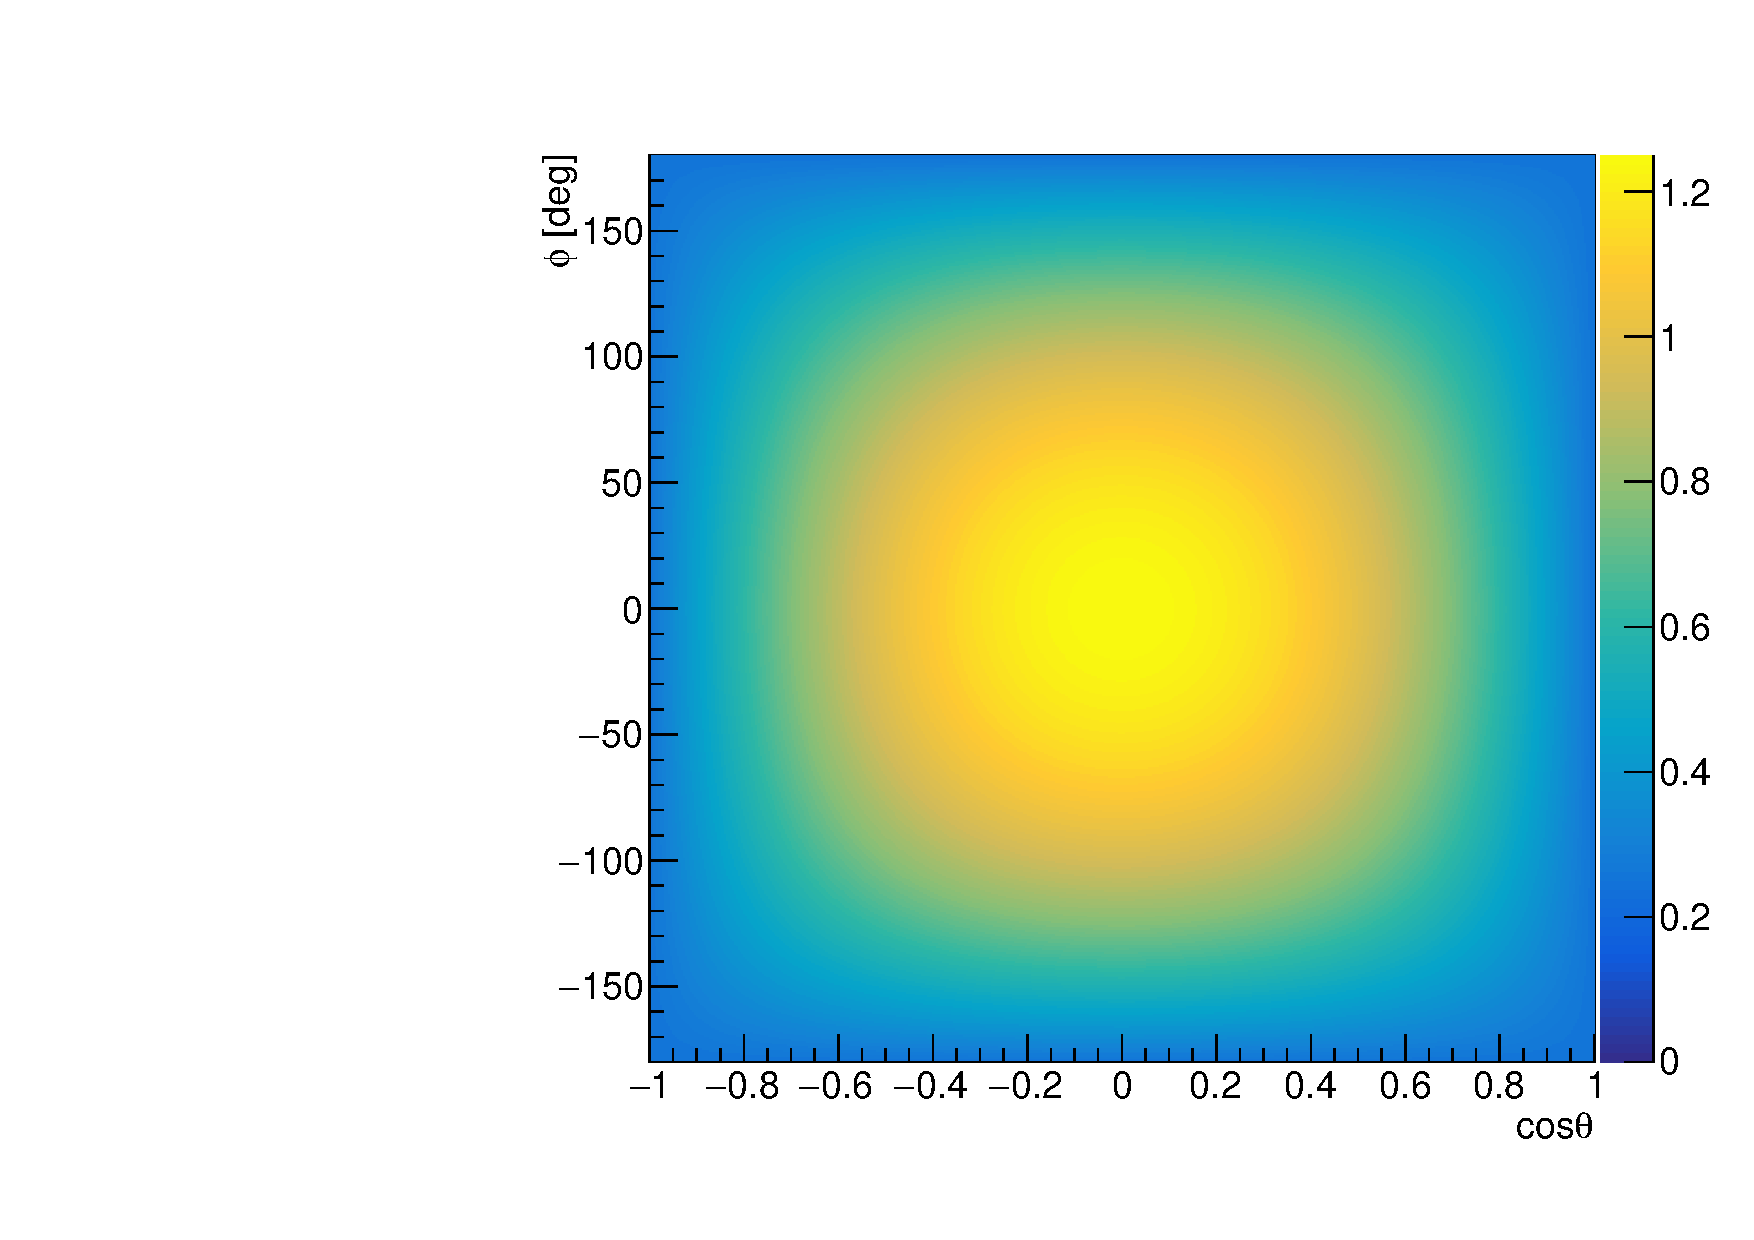
\includegraphics[width=0.5\textwidth]{diffractive/acc_4/hEfficiency}%
  }%
  \\%
  \subfloat[][]{%
    \label{fig:diffraction_study_intensity_acc}%
    \includegraphics[width=0.5\textwidth]{diffractive/acc_4/hIntensity}%
  }%
  \subfloat[][]{%
    \label{fig:diffraction_study_data}%
    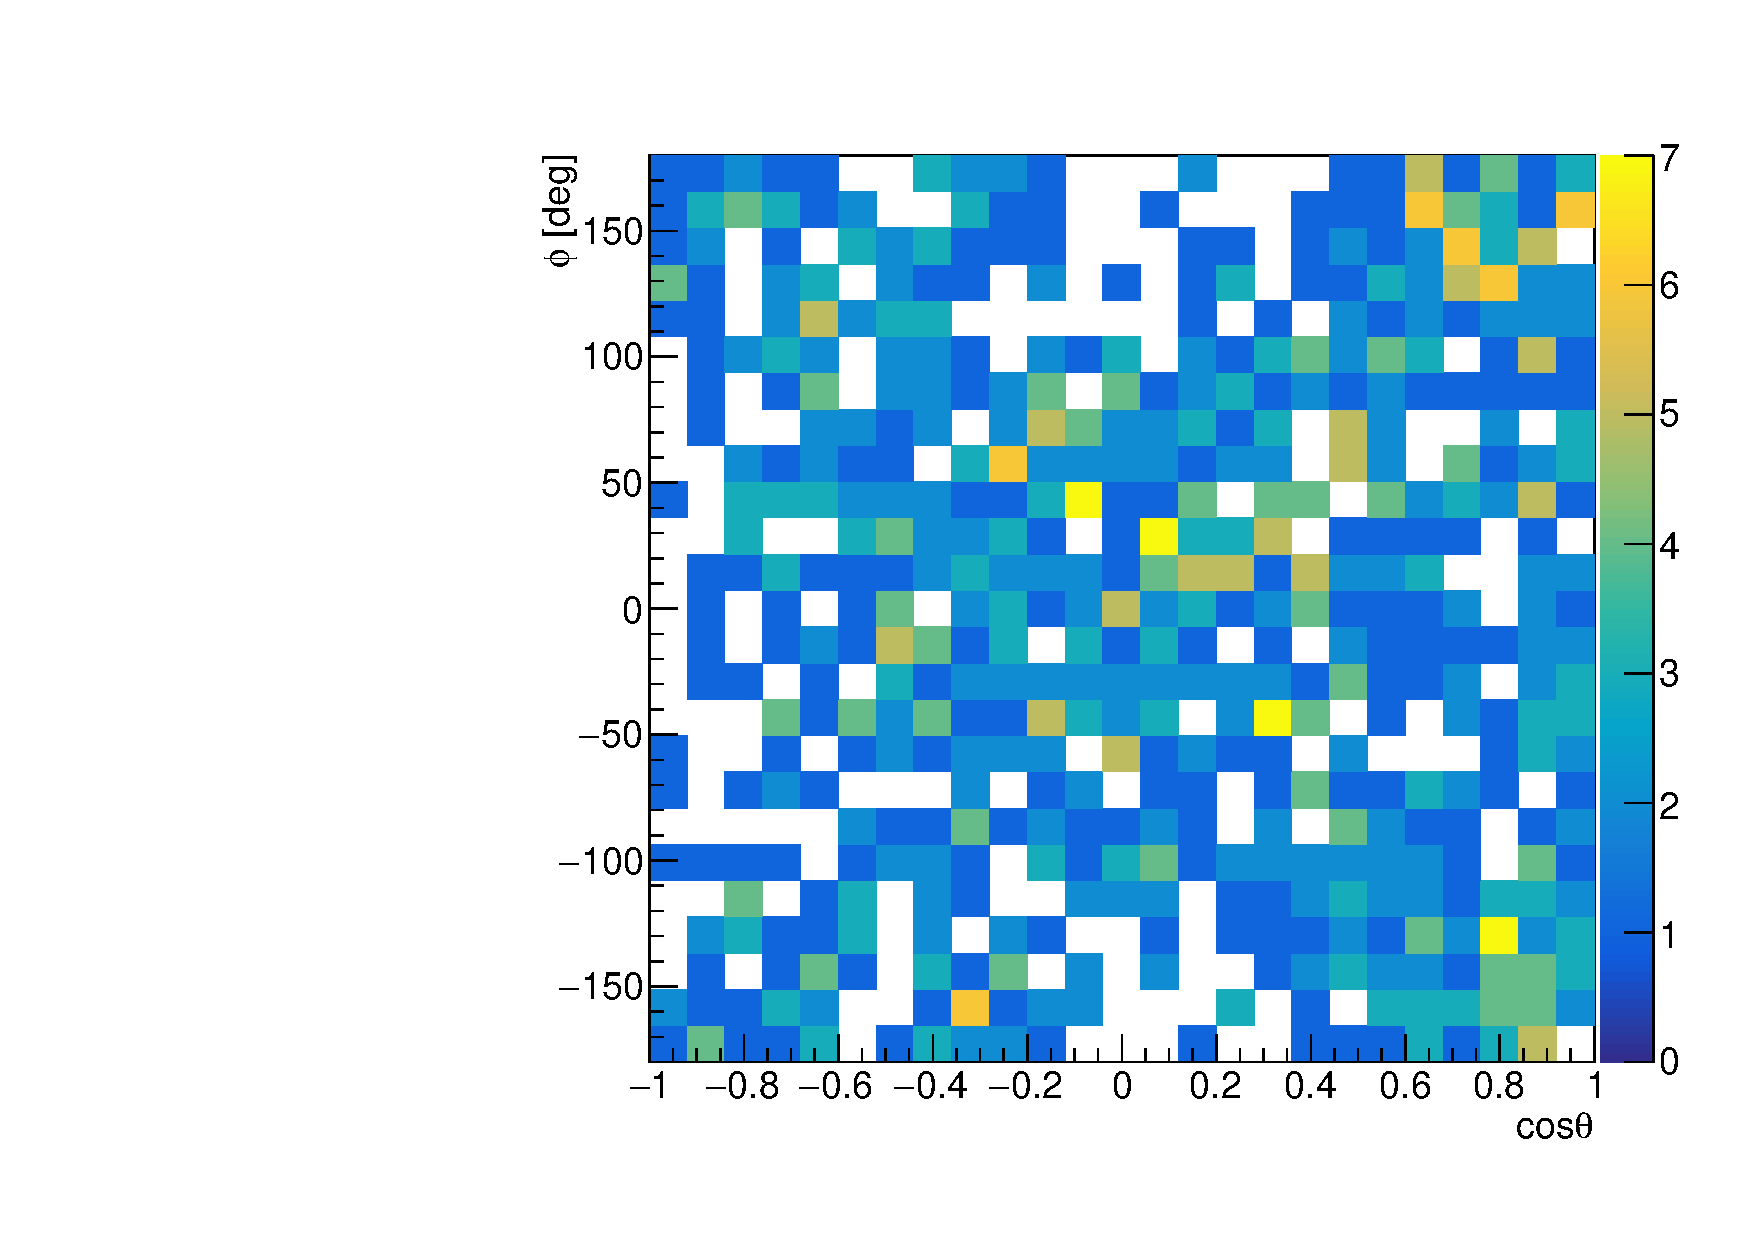
\includegraphics[width=0.5\textwidth]{diffractive/acc_4/hData}%
  }%
  \caption{Input used to generate Monte Carlo data:
  \subfloatLabel{fig:diffraction_study_intensity}~Intensity
  distribution $\intensity(\Omega)$ calculated from the partial-wave
  amplitudes listed in \cref{tab:diffraction_study_waveset}.
  \subfloatLabel{fig:diffraction_study_efficiency}~Contrived detection
  efficiency $\eta(\Omega)$ as given by
  \cref{eq:diffraction_study_acc1}.
  \subfloatLabel{fig:diffraction_study_intensity_acc}~Intensity
  distribution weighted by the detection efficiency, \ie
  $\eta(\Omega)\, \intensity(\Omega)$.
  \subfloatLabel{fig:diffraction_study_data}~Monte Carlo data sample
  of \num{1000}~events randomly drawn from the distribution
  in~\subfloatLabel{fig:diffraction_study_intensity_acc}.}%
  \label{fig:diffraction_study_input}%
\end{figure}

The acceptance integral matrix~$\mat{I}^\text{acc}$ is calculated
using \cref{eq:diffraction_integral_matrix_mc} based on \num{e7}~events
that are sampled randomly from the detection efficiency $\eta(\Omega)$
in \cref{eq:diffraction_study_acc1}.  Using this matrix, the physical
moments are calculated from the measured moments using
\cref{eq:diffraction_phys_moments,eq:complex_uncert_prop}.
\Cref{fig:diffraction_study_comparison_re} shows the physical moments
extracted from the Monte Carlo data in
\cref{fig:diffraction_study_data} and compares them to the expected
moment values calculated from the partial-wave amplitudes in
\cref{tab:diffraction_study_waveset} using
\cref{eq:diffraction_moments_pw_refl_norm}.  As expected, the two sets
of values agree within statistical uncertainties (see
\cref{fig:diffraction_study_residual_re}).  Since the physical moments
are real-valued (see \cref{eq:diffraction_moment_real}), we expect
their imaginary parts to be consistent with zero.
\Cref{fig:diffraction_study_comparison_im,fig:diffraction_study_residual_im}
show that this is true, although the scatter of the points is somewhat
larger than that of the real parts.

\begin{figure}[tbp]
  \centering%
  \subfloat[][]{%
    \label{fig:diffraction_study_comparison_re}%
    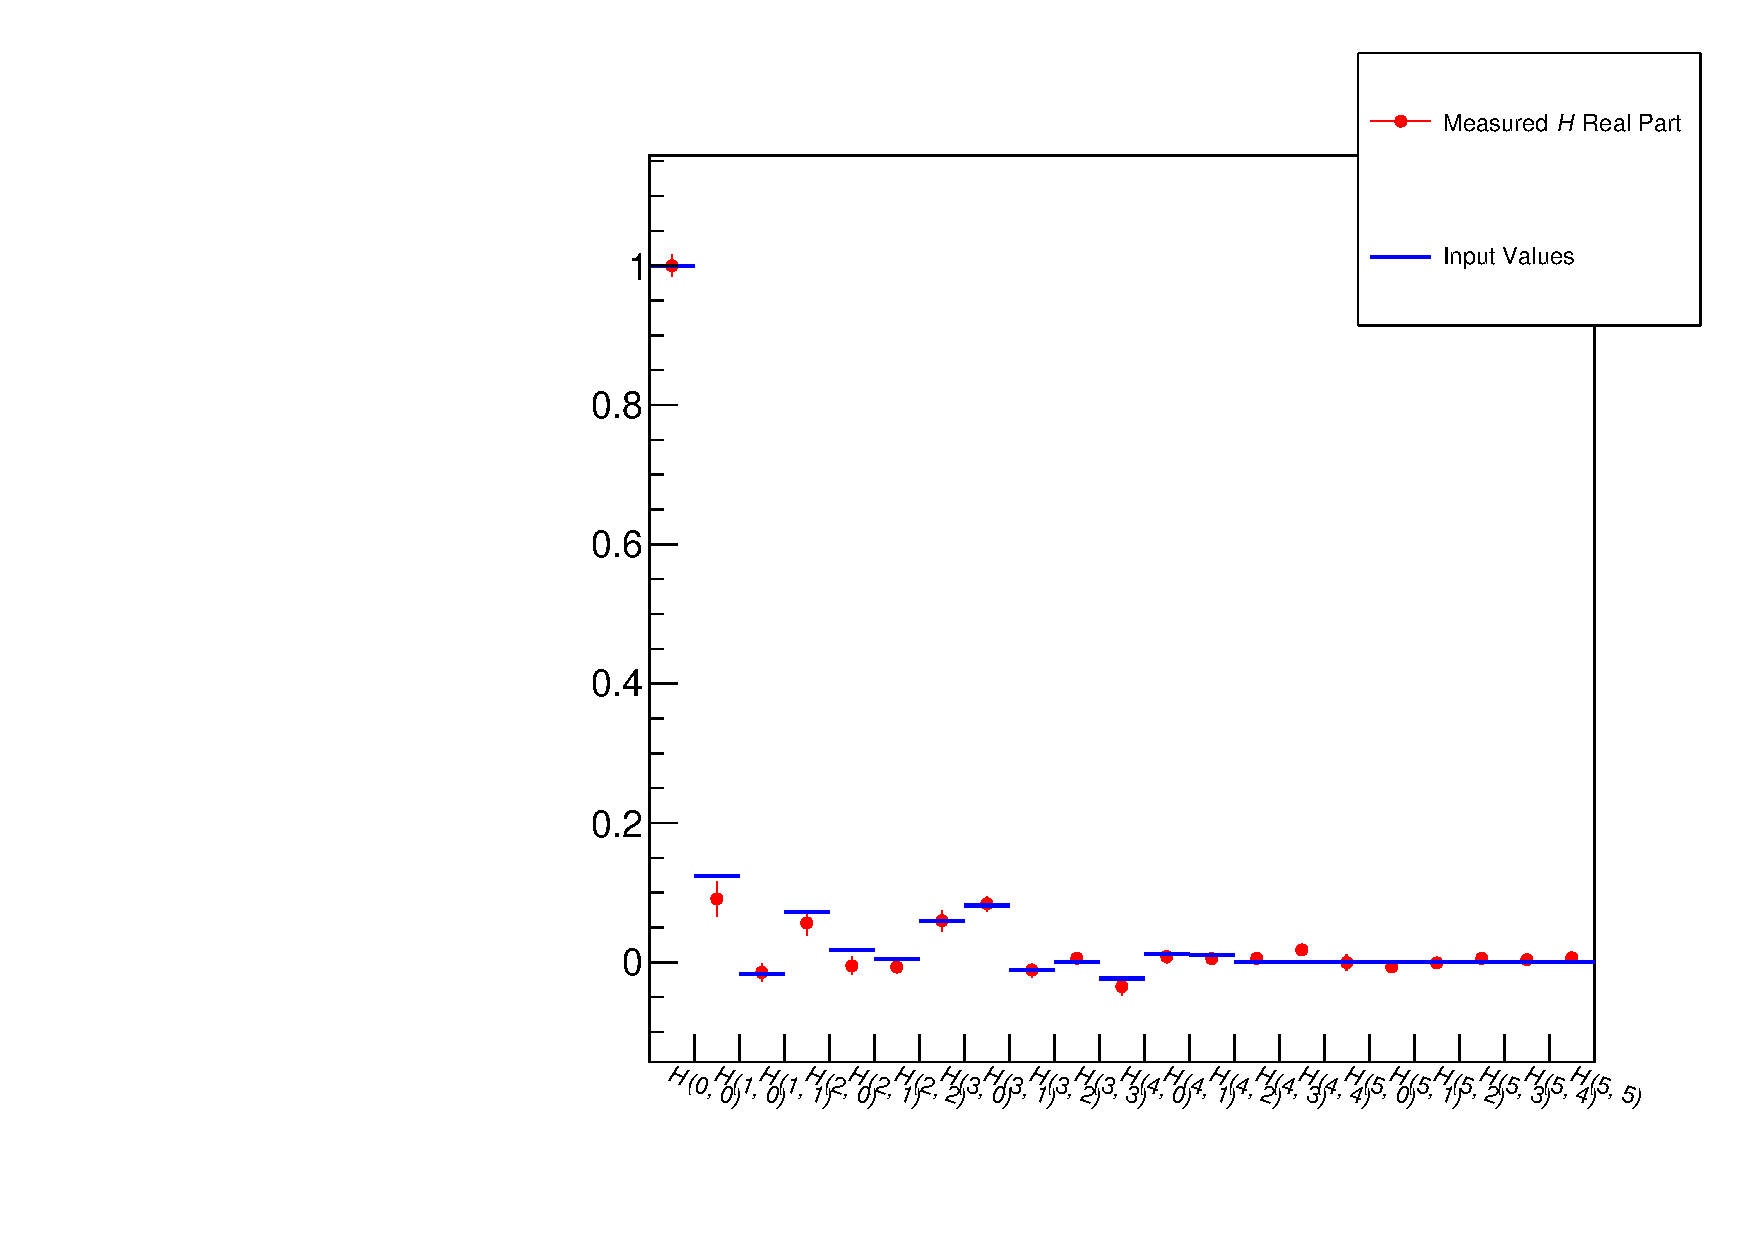
\includegraphics[width=0.5\textwidth]{diffractive/acc_4/hCompare_H_Re}%
  }%
  \subfloat[][]{%
    \label{fig:diffraction_study_comparison_im}%
    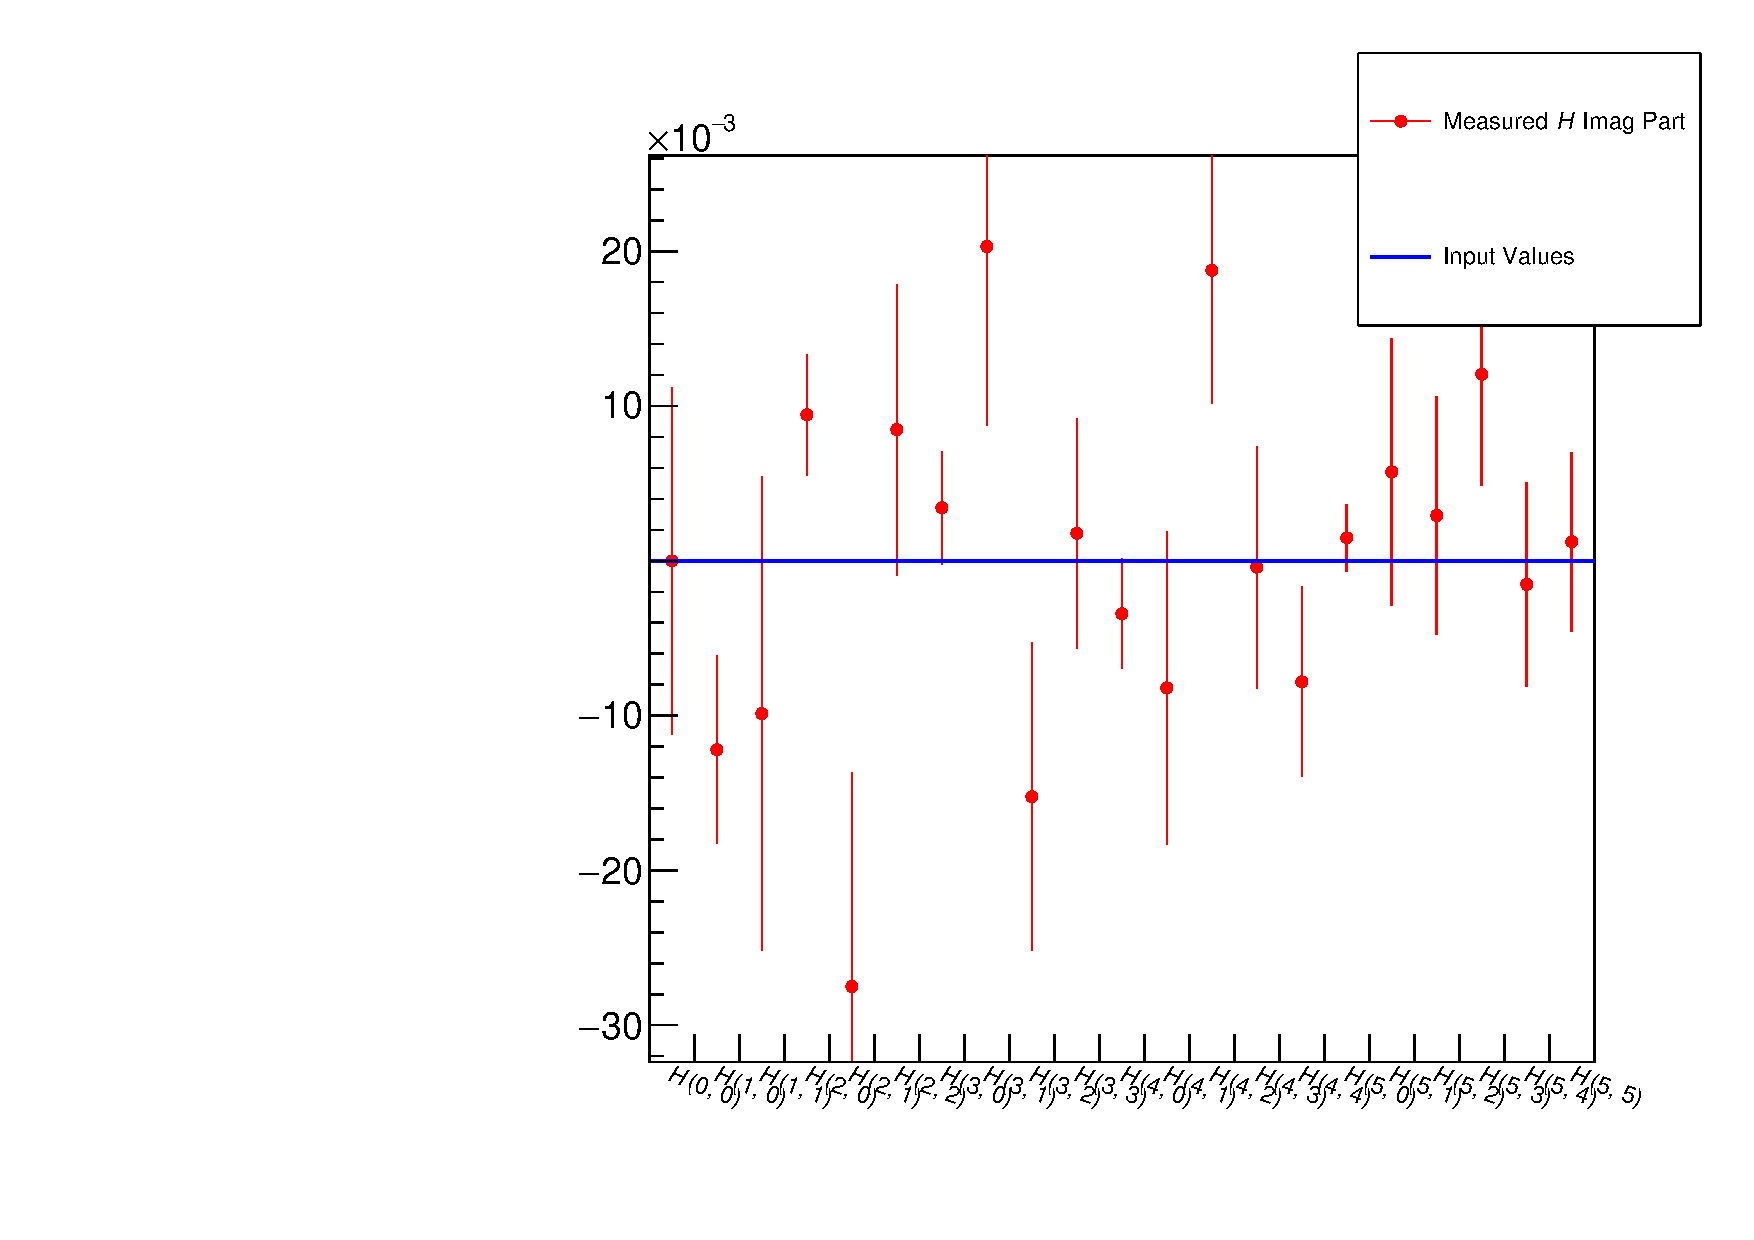
\includegraphics[width=0.5\textwidth]{diffractive/acc_4/hCompare_H_Im}%
  }%
  \\%
  \subfloat[][]{%
    \label{fig:diffraction_study_residual_re}%
    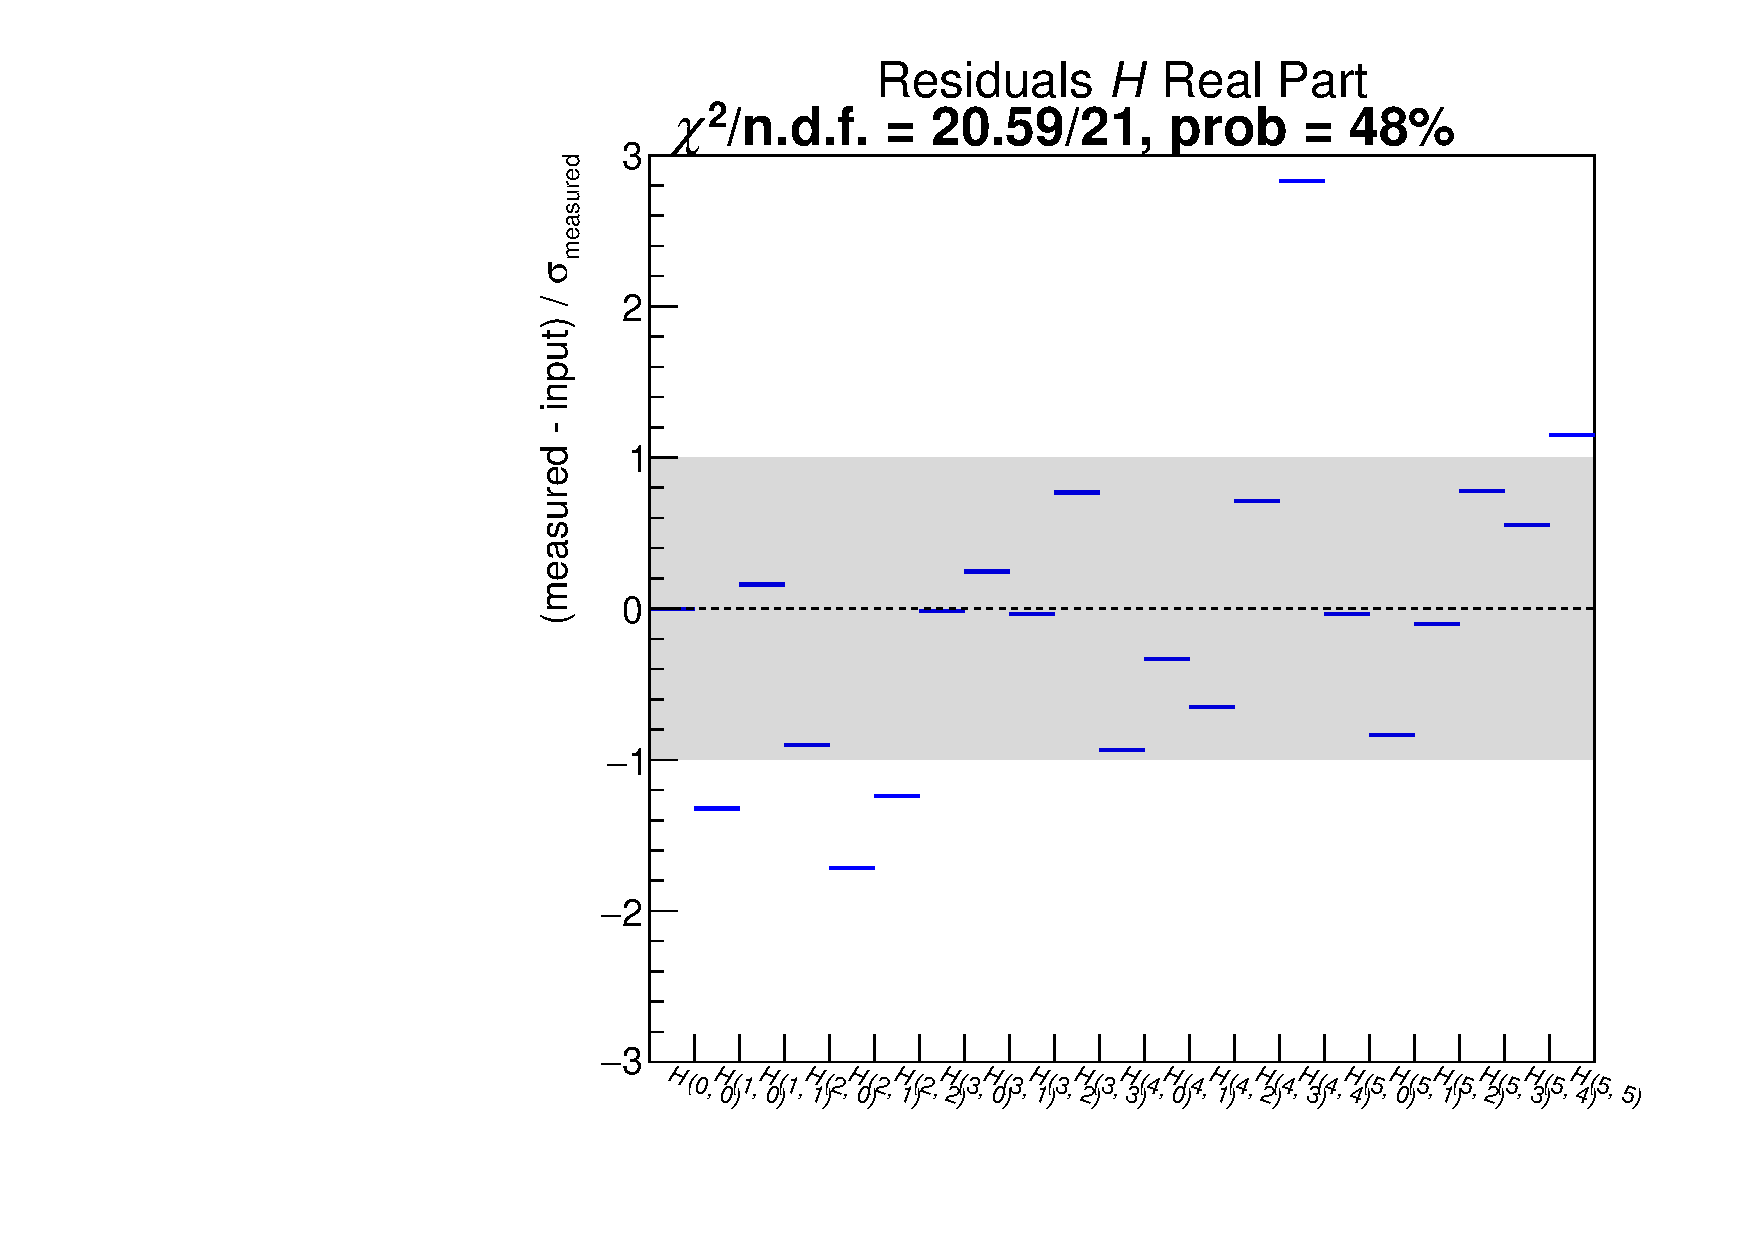
\includegraphics[width=0.5\textwidth]{diffractive/acc_4/hResiduals_H_Re}%
  }%
  \subfloat[][]{%
    \label{fig:diffraction_study_residual_im}%
    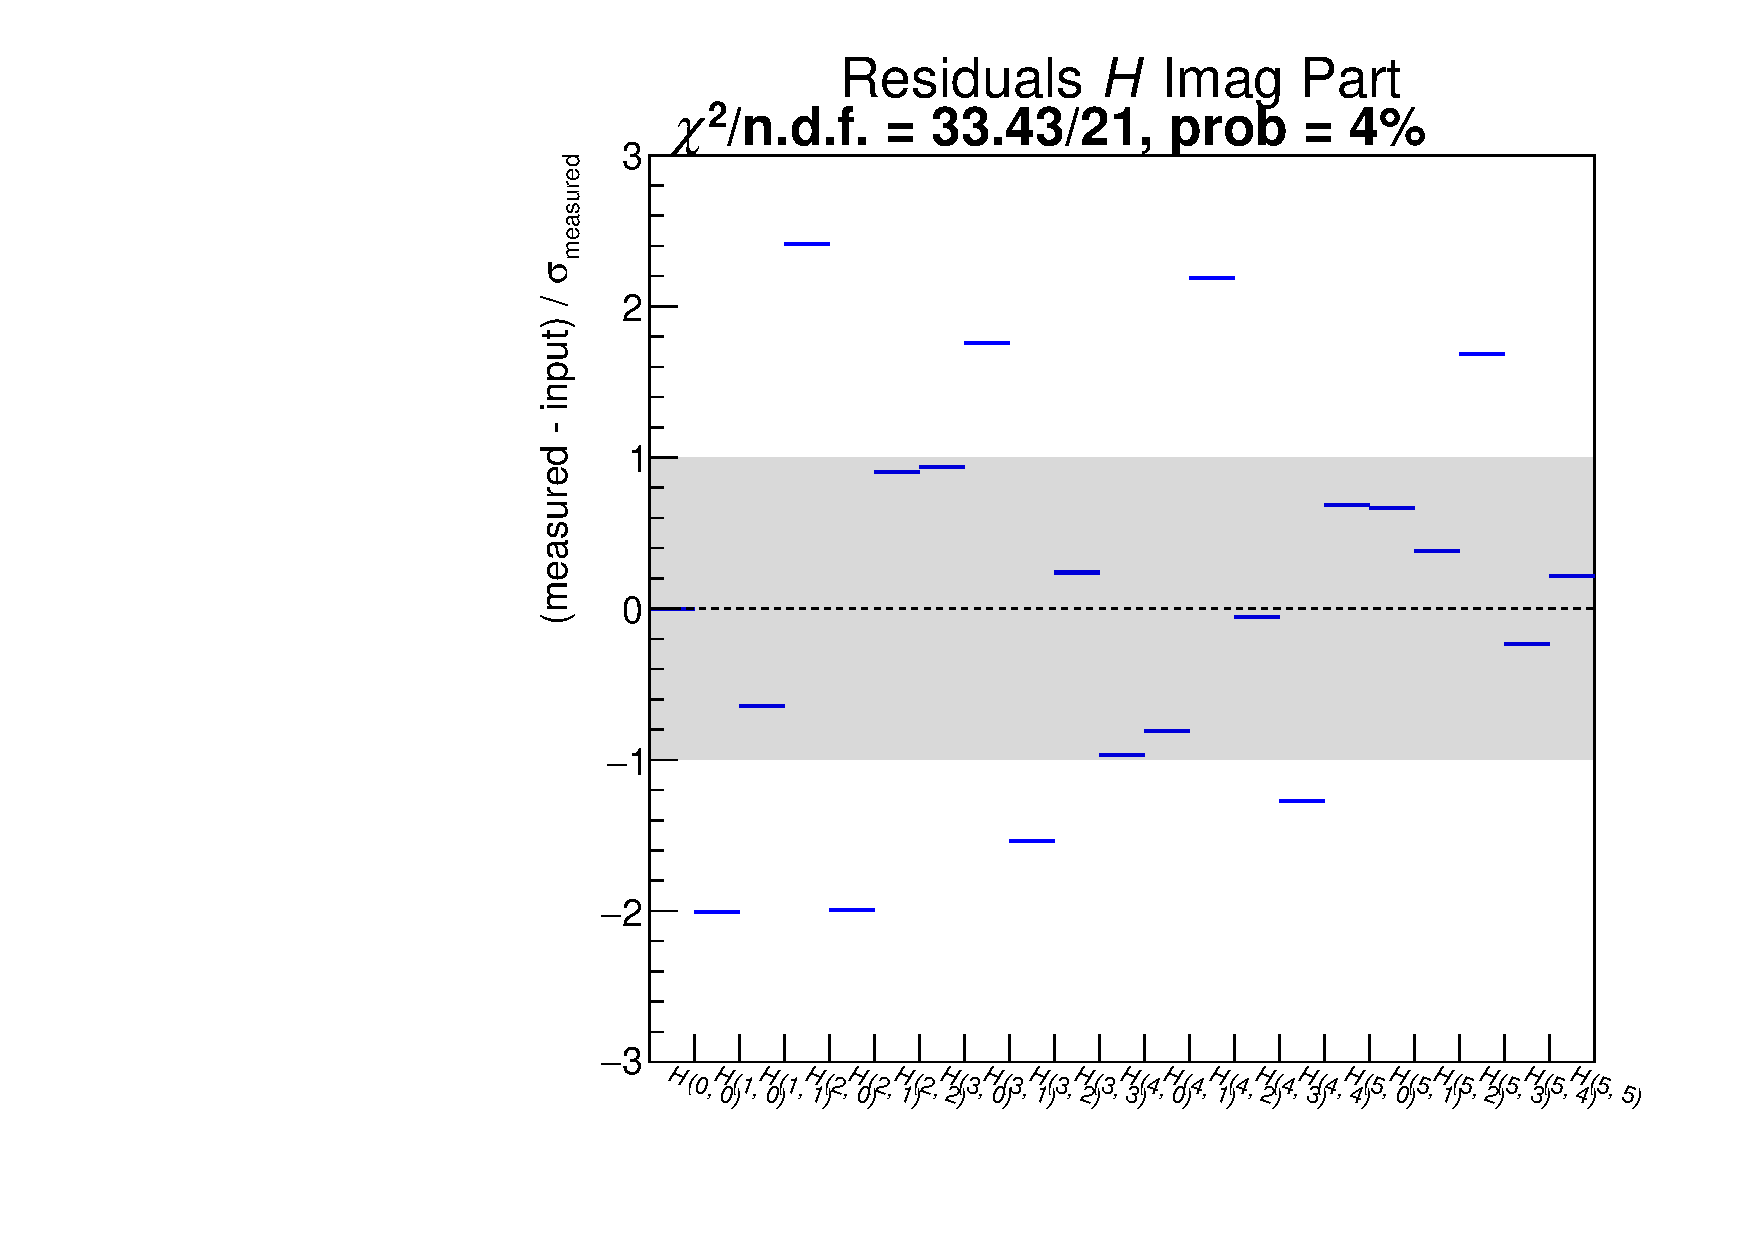
\includegraphics[width=0.5\textwidth]{diffractive/acc_4/hResiduals_H_Im}%
  }%
  \caption{Upper row: Comparison of the physical moments (red points
  with uncertainties) extracted from the Monte Carlo data, which are
  generated using the partial-wave amplitudes in
  \cref{tab:diffraction_study_waveset} and the detection efficiency in
  \cref{eq:diffraction_study_acc1}, with the expected values (blue
  lines).  Both sets of values are normalized to the value of $H_0(0,
  0)$ in the set.
  \subfloatLabel{fig:diffraction_study_comparison_re}~shows the real
  part, \subfloatLabel{fig:diffraction_study_comparison_im}~the
  imaginary part.  Note that moments with $M > 2$ and/or $L > 4$ are
  expected to be zero due to the chosen wave set.  Lower row:
  corresponding residuals.}%
  \label{fig:diffraction_study_output}%
\end{figure}

\todoInl{Discuss acceptance correction using moment decomposition of $\eta^{-1}(\Omega)$}
